% RS comment and modifications 08/01/2014 


\documentclass[12pt,a4paper]{article}
\usepackage[]{algorithm2e}
\usepackage{tabularx}
\usepackage[T1]{fontenc}
\usepackage{float}
\usepackage[latin9]{inputenc}
\usepackage{epsfig}
\usepackage{enumitem}
\usepackage{amsmath}
\usepackage{amsfonts}
\usepackage{lipsum}
\usepackage{longtable}
\usepackage{subcaption}
\usepackage{booktabs}
\usepackage{adjustbox}

%\usepackage[dcucite,abbr]{harvard}
%\harvardparenthesis{none}
%\harvardyearparenthesis{round}
%\newcommand{\citeasnoun}[1]{\cite{#1}}
\usepackage{rotating}
\usepackage{changepage}
\usepackage{csvsimple,longtable,booktabs}
\setcounter{secnumdepth}{4}
%%%%%%%%%%%%%%%%%%%%%%%%%%%%%% User specified LaTeX commands.
%\usepackage{euler,times}
%\usepackage{euler,beton}	% RS comment out - normal text font

\usepackage{lmodern}


% load titlesec
\usepackage[compact]{titlesec}
\newcommand{\sectionbreak}{\clearpage}

\titlespacing\section{0pt}{12pt plus 1pt minus 1pt}{0pt plus 2pt minus 2pt}
\titlespacing\subsection{0pt}{5pt plus 1pt minus 1pt}{0pt plus 2pt minus 2pt}
\titlespacing\subsubsection{0pt}{5pt plus 1pt minus 1pt}{0pt plus 2pt minus 2pt}

\titleformat{\paragraph}
{\normalfont\normalsize\bfseries}{\theparagraph}{1em}{}
\titlespacing{\paragraph}
{5pt}{5pt plus 1pt minus 1pt}{0pt plus 2pt minus 2pt}


%%%%%%%%%%%%%%%%%%%%%%%%%%%%%% User specified LaTeX commands.
%\usepackage{euler,times}
%\usepackage{euler,beton}	% RS comment out - normal text font

\usepackage[margin=1.3in]{geometry} % RS addition

% \newcommand{\footnoteremember}[2]{	% RS comment out - more simple affiliation
% \footnote{#2}
%   \newcounter{#1}
%   \setcounter{#1}{\value{footnote}}
% } 
% \newcommand{\footnoterecall}[1]{
% \footnotemark[\value{#1}]
% } 

\usepackage{pgfplotstable,booktabs}


\begin{filecontents*}{avg_value.csv}
Strategy,batteryCost,avgWaitingTime,maxWaitingTime,minWaitingTime,stabilityWaitingTime,averageOccupancy,averageLoadFactor,maxLoadFactor,minLoadFactor,completedBookingsRatio, ba
Constant Waiting Time at Stops,18.03,15,167,0,662,2.34,0.24,0.61,0.11,0.70,0.39
Constant Fleet Size,16.62,10,127,0,307,2.44,0.25,0.29,0.21,0.83,0.47
Optional Stops,25.92,5,57,0,36,2.87,0.29,0.40,0.15,0.81,0.63
Strategy 1: Cost Function,14.82,8,35,0,59,3.09,0.30,0.38,0.20,0.79,0.48
Strategy 2: Max Waiting Time,16.58,7,96,0,91,4.20,0.45,0.57,0.36,0.83,0.49
Spread Charging Stations,14.25,8,59,0,101,2.97,0.31,0.51,0.08,0.81,0.56
Battery Consuming Less,10.29,5,54,0,52,2.34,0.24,0.27,0.19,0.86,0.63
\end{filecontents*}


\begin{filecontents*}{values2.csv}
dem,|V|,batteryCost,avgWaitingTime,completedBookingsRatio
13,2,0.21,14,0.62
13,3,0.32,7,0.77
13,4,0.42,7,0.62
13,5,0.55,4,0.77
13,6,0.59,5,0.54
13,7,0.74,3,0.69
13,8,0.82,3,0.62
13,9,0.94,6,0.69
13,10,1.02,3,0.62
15,2,0.18,5,0.40
15,3,0.23,12,0.33
15,4,0.41,3,0.67
15,5,0.43,2,0.67
15,6,0.63,7,0.40
15,7,0.55,6,0.33
15,8,0.63,3,0.40
15,9,0.87,3,0.47
15,10,0.81,4,0.40
21,2,0.07,23,0.19
21,3,0.20,3,0.24
21,4,0.40,9,0.38
21,5,0.47,9,0.33
21,6,0.56,1,0.29
21,7,0.65,2,0.43
21,8,0.67,1,0.48
21,9,0.53,7,0.29
21,10,0.91,1,0.48
23,2,0.20,11,0.35
23,3,0.20,21,0.09
23,4,0.34,11,0.39
23,5,0.39,8,0.30
23,6,0.36,11,0.22
23,7,0.63,13,0.39
23,8,0.67,3,0.57
23,9,0.68,11,0.26
23,10,0.84,3,0.43
25,2,0.16,13,0.36
25,3,0.27,4,0.44
25,4,0.40,6,0.52
25,4,0.40,6,0.52
25,5,0.48,7,0.56
25,6,0.52,5,0.56
25,7,0.43,4,0.56
25,9,0.71,4,0.44
25,10,0.93,3,0.64
27,2,0.14,28,0.11
27,3,0.22,14,0.19
27,4,0.22,15,0.26
27,5,0.45,9,0.30
27,6,0.44,6,0.30
27,7,0.71,4,0.52
27,8,0.59,3,0.33
27,9,0.73,5,0.41
27,10,0.75,2,0.37
31,2,0.19,8,0.39
31,3,0.23,10,0.42
31,4,0.29,4,0.45
31,5,0.37,4,0.39
31,6,0.41,2,0.32
31,7,0.52,2,0.42
31,8,0.79,3,0.58
31,9,0.87,3,0.45
31,10,0.89,2,0.45
36,2,0.17,14,0.44
36,3,0.27,7,0.36
36,4,0.38,6,0.42
36,5,0.48,13,0.33
36,6,0.25,5,0.47
36,7,0.69,7,0.50
36,8,0.70,6,0.50
36,9,0.83,4,0.31
36,10,0.73,4,0.42
40,2,0.16,26,0.23
40,3,0.28,32,0.30
40,4,0.31,5,0.30
40,5,0.46,16,0.40
40,6,0.51,13,0.30
40,7,0.62,10,0.45
40,8,0.72,7,0.48
40,9,0.79,5,0.30
40,10,0.79,3,0.35
46,2,0.19,9,0.24
46,3,0.09,63,0.13
46,4,0.38,6,0.28
46,5,0.40,3,0.30
46,6,0.57,7,0.35
46,7,0.60,5,0.22
46,8,0.67,6,0.39
46,9,0.83,5,0.39
46,10,0.65,5,0.20
58,2,0.18,12,0.31
58,3,0.22,11,0.21
58,4,0.12,22,0.38
58,5,0.31,9,0.22
58,6,0.40,15,0.29
58,7,0.67,10,0.47
58,8,0.72,4,0.53
58,9,0.80,9,0.36
58,10,0.93,5,0.52
\end{filecontents*}

\usepackage[authoryear]{natbib} % package to use Harwad style for reference http://www.andy-roberts.net/writing/latex/bibliographies

\begin{document}


\thispagestyle{empty}

  \vspace{-3cm}
  
\includegraphics[height=2cm]{./images/EPFL.pdf}
%  \hspace{1.5cm} \includegraphics[height=2cm]{./images/Trace.jpg} 
  \hfill 
\includegraphics[height=2cm]{./images/bestmile.jpg}
  
  \hrulefill
  \vspace{3.0cm}

%%%%%%%%%%%%%%%%%%%
%%  TITLE HERE  %%%
%%%%%%%%%%%%%%%%%%%
\begin{center}
 Master Project 
 \LARGE
 \bigskip
 
Experimental Comparison of Autonomous Vehicles Scheduling Algorithms
\end{center}

%%%%%%%%%%%%%%%%%
%% TITLE HERE %%%
%%%%%%%%%%%%%%%%%


%%%%%%%%%%%%%%%%%%%
%% AUTHORS HERE %%%
%%%%%%%%%%%%%%%%%%%
\vspace{2.0cm}
\begin{tabbing}
\hspace*{3cm}		\=	\hspace*{5cm}							\=	\hspace*{3cm} \\
Author:			\>	Prisca Aeby		  \textsuperscript{1}	\> prisca.aeby@epfl.ch\\
Supervisors:		\>	Bastien Rojanawisut	  \textsuperscript{2}	\> bastien.rojanawisut@bestmile.com\\	
					\>	Boi Faltings    \textsuperscript{3}	\> boi.faltings@epfl.ch\\
\end{tabbing}
%%%%%%%%%%%%%%%%%%
% AUTHORS HERE %%%
%%%%%%%%%%%%%%%%%%



\begin{center}

\today
\end{center}

\vfill
\hrulefill

\small \textsuperscript{1} Computer Science,  \'Ecole Polytechnique F\'ed\'erale de Lausanne, Switzerland

\small \textsuperscript{2} Scala Backend Software Engineer, BestMile, Switzerland 

\small \textsuperscript{3} Artificial Intelligence Laboratory, School of Computer and Communication Sciences, \'Ecole Polytechnique F\'ed\'erale de Lausanne, Switzerland, \verb+liawww.epfl.ch+ 




\newpage


\begin{abstract}
Your abstract.
\end{abstract}

\newpage

\tableofcontents
\newpage
\setlength{\parskip}{0.5em}
\section{Introduction}
General problem: two types of services, on-demand and fixed-line => explain why we focus on fixed line (all constraints of the platform) 
Fixed line because now roads are not made for more complex systems
Goal: run simulations as close as possible to real world situations
=> how much it can improve the system performances to be able to forecast demand
bring concrete solution to transport models which are implemented now

\section{Related literature}\label{literature} 
The scope of vehicle scheduling problems related to our specific case study can range from fixed-line bus services to on-demand systems. In fact, routes and stops of the electric shuttles are predefined but timetables can be flexible to respond to the real-time demand. The set of constraints differs from traditional bus transportation: workforce regulations can be eliminated as the shuttles are not human driven, a battery management component needs to be introduced into the planning process (e.g. charging times need to be considered), the operational network has a different layout, etc. As we will see in this chapter, current research often concentrates on one specific aspect of the scheduling strategy, simplifying some constraints, assessing the system's performance using various types of metrics and considering different inputs. In what follows, we describe in Section \ref{pubtrans} some techniques used in the traditional public transport industry to guarantee a good quality of service. In Section \ref{das} we describe the concept of Demand-Adaptive Transit Systems. Finally, we detail in Section \ref{luts} an approach proposed by the Urban Transport Systems Laboratory (LUTS) at EPFL for scheduling autonomous vehicles activities.  

\subsection{Public transport}\label{pubtrans}
Within the standard transit organization, policies and standards affect a lot the development of strategies and how people interact with the public transports. The planning process of a fixed line bus transportation service is mainly composed of three different tasks: route planning, deciding service frequencies and defining the service timing. Route planning consists of selecting a sequence of stops composing each route and how those routes are interconnected. Deciding service frequencies implies specifying the number of vehicles per unit time which need to pass a given route (often expressed in vehicles per hour). A common measure used to express the ideal distance between vehicles is the headway, the inverse of the frequency, in other word the fixed interval at which vehicles are coming at a station. The service frequencies set by the transport organization can be chosen based on different policies (see \cite{tcrp}): 
\begin{enumerate}
\item \textbf{Fixed headway}: the agency establishes a fixed interval and time at which vehicles come to stations. It is convenient for customers as they have access to an exact schedule, but it is hard to keep the time between vehicles constant as it is vulnerable to external disturbances (e.g. traffic, stochastic passenger arrivals at stops, traffic jams, etc.).
\item \textbf{Demand-based headway}: in existing transport services, agencies can adapt the timetables based on the observed demand at the stations (number of passenger boardings/deboardings) in order to reach the desired passenger load in vehicles.
\item \textbf{Performance-based headway}: the goal is to find the headway for which performance standards are optimized. Those costs are usually measured during a service period, for example a day. It may include the service productivity (e.g. the revenue per passenger per hour), the cost effectiveness of the service or the overall effectiveness (e.g. net subsidy per passenger). 
\end{enumerate}

All those scheduling strategies suffer from the well-known bunching effect: two or more buses arrive at the same time at a stop with the first one being overcrowded and the other ones empty. This phenomenon occurs because of external disruptions in the service (see \cite{hwadherence}) slowing down one of the bus which pick up passengers who would have normally taken the next bus. 

Several corrective measures based on different strategies have been developed to overcome this problem. There are mainly two different holding approaches to mitigate bus bunching as described in \cite{reliability}:

\begin{itemize}
\item \textbf{Headway-based holding:} vehicles arriving with a shorter headway at a stop (or holding point) wait to restore the headway distribution. If they arrive with a longer headway, it is possible to speed up the buses by skipping stations. The analytical study \cite{hybrid} proved the efficiency of using headway holding strategy and bus skipping (considering the extra waiting time of passenger whose station has been skipped) with a two-dimensional objective function composed of the regularization of bus headway on the one hand and the level of service on the other hand with respect to a circular route scenario. 
\item \textbf{Schedule-based holding:} in the case of fixed timetables, schedule-based holding involves holding a vehicle at a stop if it is ahead of its schedule and dispatch it immediately otherwise.
\end{itemize}
  
\cite{selfadjusting} proposed a method using boarding limits at stations to control buses which does not involve bus accelerating or waiting at stations and thus does not influence the customers' travel time and does not disturb the traffic. They do not consider a fixed schedule and a priori target headway. However, they proved that their self-adjusting control stabilizes the headway spontaneously in a short time. 

As stated by \cite{information}, the majority of earlier studies conducted on maintaining a balanced headway uses arrival time of the current bus at the current stop and arrival times of the preceding buses but does not take advantage of real time information like the vehicles' geolocation. Later methods proposed new approaches assuming availability of locations and even real-time arrivals of passengers to each bus stop. For example, \cite{cooperation} proposed a solution taking into account the distance between the current bus and the preceding and following buses to adjust the speed of the current bus. It includes holding buses at stations, accelerating or decelerating. 

An important measure used in public transport in addition to the headway is the load factor. The passenger load factor measures the efficiency of a transportation system, representing the capacity utilization of the seats. It is often expressed as the ratio between the passenger-kilometers travelled to seat-kilometers available. For example \cite{loadFactor} study the importance of the vehicle load effects on the emission of vehicles through the study of the load factor and the empty running rate. They discuss the variation of the factor with various parameters (e.g. vehicle size, vehicle weight, time, travel purpose).

The studies carried out within the traditional fixed-line bus services handle situations where the demand is consistently strong over the territory and where the fleet is composed of high-capacity vehicles. When the demand is weaker, it is complicated to operate an economical and frequent transit system as the resources are shared by few people and are very costly (e.g. driver salaries, fuel expenses, etc.). The autonomous fleets are composed of vehicles with lower capacity, but it is easier to dynamically adapt their scheduling strategy at low cost and have access to real-time information.

\subsection{Demand-adaptive transit systems}\label{das}
Demand-Adaptive System (DAS), or Demand-Responsive Transit (DRT), is a personalized type of transportation displaying features from both fixed-line services and on-demand systems. The line is often designed as a loop with some mandatory stops, and the trajectory of the buses can be adapted between two mandatory stops to serve passengers at additional optional stops. There compulsory stops are served within a predefined time window. A method to determine those time windows has been proposed by \cite{masterschedule}: they use a  solution framework based on decoupling the origin-destination demand with a cooperative-search algorithm. \cite{dasdesign} depicted the advantages to substitute fixed-line bus services to DRT services in two cities in California with low demand density. They propose a strategy substituting the current fixed line bus service to a demand responsive transit line and show that 2 buses instead of 4 could serve the demand. 

\cite{evaluation} address the issues of evaluating DAS services in comparison to traditional transit services and fully on-demand systems. The transit evaluation denotes the part of the planning process dedicated to the study of the behaviour and the performance of the line under various conditions with respect to demands, policies and costs. They mention the main steps of transit lines' evaluation in order to tune operating parameters impacting the system performance under different scenarios for cost-benefit analyzes: 
\begin{enumerate}
\setlength\itemsep{1pt}
\item the scenario, parameters and policies are specified, as well as the demand to serve
\item the line is designed
\item the operation of the line is simulated (during a specified time-horizon)
\item results are collected and performance measures are computed. 
\end{enumerate}
The importance of demand generation in step 1) differs from one system to the other: whilst in fixed lines transits static methods are often used to simulate an average demand, dynamic methods are used to simulate the time-dependent stop-to-stop requests in on-demand transport services. The performance measurements in step 4) vary as well from one system to the other: in fixed-lines the service quality is mainly represented by the punctuality of the buses and the constant interarrival times whereas for on-demand services it is expressed by the specific users' waiting time and excess riding time. \cite{evaluation} propose a framework for evaluating DAS lines including the scenario input, the optimization modules for the design and operation of the line and the simulation module which yield the statistical information about the performance.

\subsection{Vehicles assignment to routes}\label{luts}
\cite{luts} present an optimization approach for the autonomous vehicles scheduling within a transit system composed of circular routes. They separate the planning process in two main tasks: line planning and vehicle scheduling. Line planning corresponds to defining the routes and the required headway on each route over the planning horizon. Vehicle scheduling refers to computing a general assignment plan for each vehicle for each time period over the planning horizon of one day. It means that each vehicle is assigned to a specific route or to a recharging station for each time period. The underlying assumption is that the vehicles will not transfer between routes and charging stations too often which makes the time discretization of the planning horizon possible. They focus on the vehicle scheduling task which takes as input the predefined routes, headway, fleet size and battery model. They present the scheduling problem as a mixed-integer linear programming (MILP) with battery constraints and the goal of the objective function being to maximize the total battery charge levels at the end of the planning horizon (i.e. ensure the reuzability of the fleet). 

\cite{ga} tackle in their study the optimal fleet size distribution of a transit network composed of several lines and the scheduling strategy to adopt which minimizes the waiting time of passengers at their point of origin and the transfer times from one route to an other. They formulate the problem as a non-linear mixed integer programming problem (NLMIP) with resource limitations and service related constraints such as the fleet size, a minimum required headway, a minimum fleet size on each route and a maximum transfer time for passengers. They consider in the objective function only the level of service offered to the passengers, taking into account the initial waiting time of passengers and the total transfer time of passengers but no vehicles' operating cost. They mention the lack of work on this topic, possibly because of its extreme complexity, but consider the most promising attempts at solving the optimal scheduling problem being the ones using simple binary genetic algorithms as the optimization tool. 

Several aspects of our autonomous vehicles scheduling problem can relate to the literature subjects listed in this section. However, no mathematical formulation describes exactly all the constraints to consider for an autonomous electric fleet of vehicles with dynamic bookings on a closed circular line. Optimization formulations simplify many real-world constraints (e.g. schedule when to send vehicles to charge, what are the exact bookings, etc.) based on the parameters to optimized (e.g. headway, satisfy on-demand bookings, optimal fleet size, etc.). We need therefore too combine some specificity of fixed line and on-demand transportation formulations with an additional battery scheduling component.  

\section{Problem formulation}
In this section we formulate our mathematical model describing the autonomous vehicles circular line transit. All the variables are listed in Table \ref{table:parameters}. In addition to traditional bus transit system descriptions, we introduce the concept of battery stations and we include dynamic bookings from one station to an other station on the loop. We will see in Section \ref{metrics} that we have access to discrete information about the state of vehicles and bookings during the simulations. We formalize the timestamps at which  e have access to information during the service horizon time $H$, we denote a discrete timestamp $t$ which takes values between $[0, H]$ at fixed sampling $interval$.
\begin{table}
\makebox[\textwidth][c]{
  \centering
\begin{tabular}{| l | l |}
  \hline			
  Notation & Signification \\
  \hline		
  $S = \{1,..., n\}$ & Set of stations on the route \\
  $E =  \{n+i,..., 2n\}$ & Set of directed edges linking the stations \\
  $V = \{1,..., v\}$ & Set of vehicles composing the fleet \\
  $V^{\#} \subset V$ & Set of active vehicles (not charging) \\
  $C \subset S$ & Set of charging locations \\
  $B = \{1,... b\}$ & Set of bookings made during the scheduling horizon \\
  $B^{*} \subset B$ & Set of bookings which have been satisfied at the end of $H$\\
  
  $H$ & Length of the scheduling horizon \\
  $ \mathrm{interval} \in \mathbb{R}$ & Interval at which values are sampled \\
  $T = \{t = interval * k, k \in \mathbb{N} | 0 < t < H\}$ & Set of timestamps at regular $interval$ \\
  $T^{*} = \{t^{*} = 1\text{h} * k, k \in \mathbb{N} | 0 < t < H\}$ & Set of hourly timestamps \\
  $c^{v}$ & Maximum load capacity of vehicle $v \in V$\\
  $q^{v}$ & Maximum charge of vehicle $v \in V$\\
  $\alpha^{v}$ & Battery recharge rate of vehicle $v \in V$\\
  $\beta^{v}$ & Battery consumption rate of vehicle $v \in V$\\
  $s^{v}$ & Maximum speed of vehicle $v \in V$ \\
  
  $speed^{e}_{t}$ & Speed of edge $e$ at time $t$ \\
  $I^{v}_{t} \in [0, q^{v}]$ & Battery level of vehicle $v$ at time $t$ \\  
  $\Delta^{v}_{t}$ & Battery change between $t$ and its preceding timestamp \\  
  $e^{v}_{t}$ & Edge $e \in E$ which vehicle $v$ is traversing at time $t$ \\
  $next^{v}_{t}$ &  Distance to the next vehicle in front of $v$ on the loop at time $t$ \\
  $o^{v}_{t} \in [0, c^{v}]$ & Number of passengers in vehicle $v$ at time $t$ \\
  $wait^{v}_{t}$ & Seconds vehicle $v$ needs to stop at time $t$ \\  
  
  $b_{i,j} \in B$ & Request of trip from station $i$ to station $j$, $i,j \in S$ \\
  $t^{b}$ & Time at which the request $b \in B$ has been made \\
  $n^{b}$ & Number of passengers for booking $b \in B$ \\
  $p^{b}$ & Pick-up timestamp of booking $b$ \\
  $d^{b}$ & Drop-off timestamp of booking $b$ \\
  $w^{b}$ & Waiting time of booking $b$ \\
  $\rho^{b}$ & Journey time of booking $b$ \\
  $dem_{t^{*}}$ & Demand density, bookings made between $t^{*}$ and $t^{*} + 1\text{h}$\\
  $len$ & Total length of the circular route \\

  $A^{s}, s \in C$ & 1 if $s$ is an available charging station, 0 otherwise \\
  $M^{s}$ & 1 if $s$ is the stop is mandatory, 0 otherwise \\
  $1_{V^{\#}}(v,t)$ & 1 if the vehicle $v$ is active and not charging at time $t$ \\
  $1_{B^{*}}(b)$ & 1 if request $b$ has been satisfied \\
  \hline  
\end{tabular}
}
\caption{Problem sets and parameters.}
\label{table:parameters}
\end{table}
\subsection{Circular Route}
The circular line in this transportation system is a route which starts at a certain station, traverses other stations once and terminates at the starting station. The route is represented by set of stations  and a set of directed edges $E$ linking each station $s \in S$ to its following station. The set of charging stations $C$ includes stations located on the stops within the loop: $C \subset S$. If the charging station is not used by any vehicle of the fleet we have $A^{s} = 1$. A stop $s$ can be mandatory (vehicles always stop when they reach the stop) or optional (the stop can be skipped). If the stop is mandatory the boolean variable $M^{s}$ is set to 1, and 0 otherwise. The maximum speed of an edge, representing the traffic at time $t$, is expressed as $speed^{e}_{t}$. The total distance of the circular line is given by $len$.

\begin{figure} 
  \centering
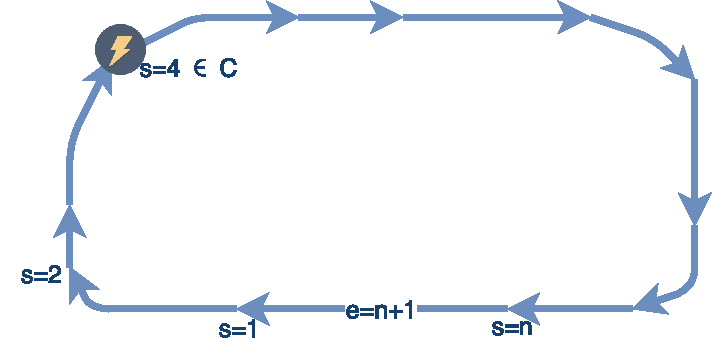
\includegraphics[scale=0.7]{./images/loop.pdf}
\caption{Example of a circular route.}
\label{fig:route}
\end{figure}

\subsection{Vehicles}\label{vehicles}
Each vehicle composing the fleet $v \in V$ moving on the circular closed line is characterized by a capacity $c^{v}$, a maximum charge $q^{v}$, a recharge rate $\alpha^{v}$, a battery consumption rate $\beta^{v}$ and a maximum speed $s^{v}$. The battery level of vehicle $v$ at the timestamp $t$ is $I^{v}_{t} \in [0, q^{v}]$. The battery change between the preceding timestamp and the current timestamp $t$ is given by $\Delta^{v}_{t}$. The edge it is currently traversing is $e^{v}_{t}$ and the distance to the next vehicle in front of it on the loop is given by $next^{v}_{t}$. The occupancy of the vehicle is expressed as $o^{v}_{t} \in [0, c^{v}]$. The vehicle is travelling either at its maximum speed or at the limitation of the current edge. Its current speed is therefore max$\{s^{v}, speed^{e^{v}_{t}}\}$. When a vehicle is charging at a station $1_{V^{\#}}(v,t) = 0$ and it can not carry any passengers $o^{v}_{t} = 0$. A vehicle entering a station at time $t$ might by forced to wait $wait^{v}_{t}$ seconds.

\subsection{Bookings and Demand}\label{bookings}
The set $B$ represents the users' bookings made during the service horizon. A booking $b_{i,j} \in B$ requests a trip from station $i$ to $j$ at time $t^{b}$ for a group of $n^{b}$ persons. If the booking has been satisfied, the boolean variable $D_{b}$ is set to 1 and we know that it has been executed by vehicle $v^{b} \in V$. The pickup time of booking $b$ at station $i$ is $p^{b}$ and drop-off time at station $j$ is $d^{b}$. The waiting time $w^{b}$ equals $p^{b} - t^{b}$ and the journey time $\rho^{b}$ is $d^{b} - p^{b}$. We denote $B^{*}$ the set of bookings which have been satisfied, so the bookings for which $1_{B^{*}(b)} = 1$. Moreover, we define the demand density $dem_{t^{*}}$ the number of bookings which have been made between $t^{*}$ and $t^{*} + 1\text{h}$, so we have $dem_{t^{*}} = |B^{\#}|$, with $\forall b \in B^{\#}: t^{*} \leq t^{*b} < (t^{*}+1\text{h})$. $t{*}$ is a discrete hourly timestamp over the scheduling horizon: $t^{*} \in T^{*}$ with $T^{*} = \{t^{*} = 1\text{h} * k, k \in \mathbb{N} | 0 < t^{*} < H\}$.

\subsection{Output Metrics}\label{metrics}
At the end of the service horizon $H$, several metrics can be derived in order to evaluate the performance of the overall system dispatching the vehicles to serve the requests. 

\subsubsection*{Battery}
The total battery consumed by a vehicle $v$ is the sum of the battery changes over the scheduling horizon when the vehicle is not charging:
$$battery^{v} = \sum_{t \in T}\delta^{v}_{t} * (1_{V^{\#}}(v,t)) $$
The total battery cost for the entire system is therefore the sum of the battery consumption of each vehicle composing the fleet:
$$batteryCost = \sum_{v \in V}battery^{v}$$
\subsubsection*{Occupancy}
The average occupancy of a vehicle $v$ over the scheduling horizon $T$ is given by:
$$avgOccupancy^{v} = \frac{\sum_{t \in T}o^{v}_{t}}{|T|}$$
The average occupancy does not take into account the time vehicles spend at charging stations and therefore can not carry any passenger. As explained in section \ref{pubtrans}, a common unit used in transportation  measurement is the load factor, which expresses the efficiency of a vehicle based on the kilometers traveled by passengers over the total kilometers that could have been driven considering its maximum capacity. In our case, as we are mainly interested in how the battery of the vehicles has efficiently been used, we define the passenger-battery measure: it is the battery that has been consumed by the vehicle during the passenger journey time. The passenger-battery for one vehicle is therefore the sum of the passenger-battery of the bookings it has satisfied. The seat-battery available represents the maximum possible passenger-battery if the vehicle would have been always full: it is the battery consumption of the vehicle times its maximum capacity. The vehicles' load factor is its passenger-battery over its seat-battery:
$$loadFactor^{v} = \frac{\sum_{t \in T} \Delta^{v}_{t} * (1_{V^{\#}}(v,t)) * o^{v}_{t}}{battery^{v} * c^{v}}$$
We can compute the average load factor of the fleet as:
$$avgLoadFactor = \frac{\sum_{v \in V}loadFactor^{v}}{|V|}$$
We measure the variance of the $loadFactor$ which expresses the stability of the occupancy among the vehicles composing the fleet. The closer it is to 0 the better as it implies that all vehicles are used equivalently: $stabilityLoadFacptr = \widehat{Var}(loadFactor)$.
%We denote the stability load factor the difference between the maximum load factor among the vehicles composing the fleet and the minimum one. The closer it is to 0 the better as it implies that all vehicles are used equivalently: $stabilityLoadFactor = \max_{v^{+} \in V}{loadFactor^{v^{+}}} -  \min_{v^{-} \in V}{loadFactor^{v^{-}}}$.
\subsubsection*{Waiting Time}
The average waiting time among the satisfied bookings is given by: 
$$avgWaitingTime = \frac{\sum_{b \in B^{*}}w^{b}}{|B^{*}|} $$
The variance of the waiting time as well which expresses the stability of the waiting time over all the bookings. As we want the waiting time to be as stable as possible we want to minimize $stabilityWaitingTime = \widehat{Var}(w)$.

\subsubsection*{Journey Time}
The average journey time among the satisfied bookings is given by:
$$avgJourneyTime = \frac{\sum_{b \in B^{*}}\rho^{b}}{|B^{*}|} $$

\subsubsection*{Completed Bookings Ratio}
At the end of the scheduling horizon, some bookings may not have been satisfied. The ratio of bookings which have been satisfied is given by:
$$completedBookingsRatio = \frac{|B^{*}|}{|B|}$$

\section{Methodology}
In order to evaluate the behaviour and performance of the system under various conditions with respect to the line configurations, the booking scenarios and the vehicles scheduling alternatives, we undertake analyses under laboratory conditions by simulating the operation of the system on the platform dispatching the vehicles. One of our main goal in the analysis we conduct on the line is to get measures as close as possible to real world conditions. In order to achieve this, a dynamic system is required which handles the time-dependent events of the system. In section \ref{framework} we describe the behaviour of the different interconnected services simulating the vehicles' behaviour reacting to external conditions and how the overall system is evaluated. In section \ref{scheduling} we present the variations of scheduling strategies used to dispatch the vehicles on the line. The parameters characterizing the simulation framework and the ones introduced in the scheduling strategy are summarized in table \ref{table:simparametersused}. 

\subsection{Simulation Framework}\label{framework}
\setlength{\belowcaptionskip}{10pt}
\begin{figure} 
  \centering
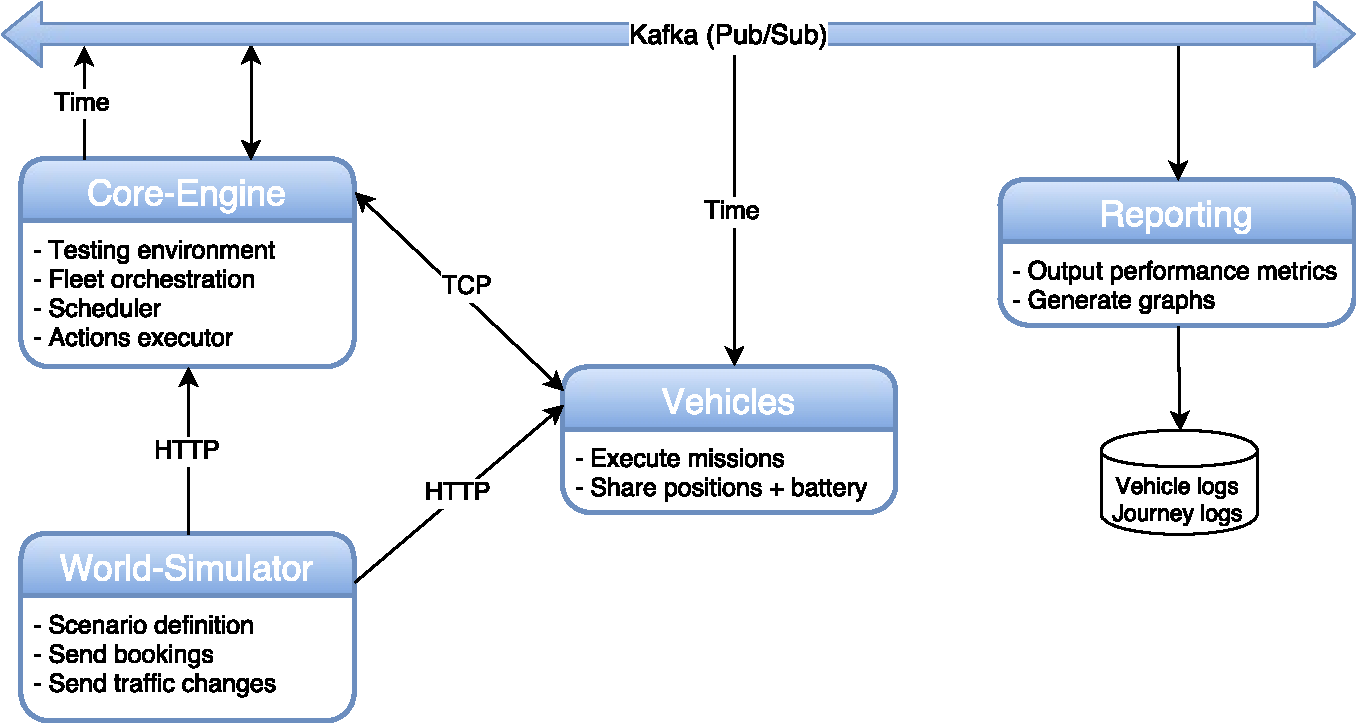
\includegraphics[scale=0.55]{./images/SimulationFramework2.pdf}
\caption{Interconnected modules composing the simulation framework.}
\label{fig:simulationFramework}
\end{figure}

Figure~\ref{fig:simulationFramework} illustrates the different web services and how they are linked to each others. Services can communicate by exchanging messages via Kafka which is an asynchronous publish-and-subscribe message broker. In what follows we describe the behaviour of each module and the simulation parameters which can be tuned. 

\subsubsection{World-Simulator}
The world-simulator is a web service which is used to start the simulation, send the booking requests and send traffic updates information through the HTTP connection established with the core-engine application. At the beginning of the simulation, it sets the time control to a given ratio which is sent to the core-engine application. A day can be simulated in $m$ minutes which corresponds to a ratio $r$ of $m / 24h$. The simulated time $simTime$ is therefore $r$ times the real time. The world-simulator is instantiated with a scenario describing the external events which affect the overall system. It mimics the bookings which would have been made by users with the booking application and sent through a REST API. Every simulated second at time $simTime$ it checks if there are bookings with $t^{b} = simTime$ and speed updates to send to the core-engine application with $speed_{t}^{e}, t = simTime$. 

\subsubsection{Simulated Vehicles}\label{simvehicles}
Vehicles are connected to the core-engine through an established TCP protocol. They can send status messages and receive missions, like going to a specific charging station or waiting at a stop at for $wait^{v}_{simTime}$ seconds. A vehicle executes every mission it receives from the core-engine. The vehicles are simulated concurrently following an actor model. Each vehicle is a different actor part of the actor system. When the vehicles web service receives an HTTP request to start the simulation with a given fleet size from the world-simulator, an actor is created for each vehicle, which announces its position to the core-engine through a TCP message and subscribes to the time topic. The vehicles start at equal distance of each others on the loop with the battery completely recharged and their position and battery level is then updated every $1000/rate$ milliseconds.  

\subsubsection{Core-Engine}
The core-engine application is a distributed system that combines and processes real-time information for coordinating and optimizing the fleet of autonomous vehicles. Several testing environment components are instantiated by the core-engine application: the map, the vehicles' configurations and fleet schedule through the day. The map is a GeoJSON file generated with QGIS, a software to create and edit geospatial information, which models the fixed line as segments of four meters. This file is then translated into the application to a directed graph with an edge between every stop and charging stations. The vehicles' configurations include all the parameters enumerated in section \ref{vehicles}. The core-engine handles the bookings it receives from the world-simulator, updates the edges' speed of the graph and sends the actions to be executed by the vehicles. When it receives the starting simulation time and ratio $r$ from the world-simulator, it publishes the updated time to the corresponding Kafka topic. The scheduler component manages the number of vehicles which need to be on service at different times during the day and sends corresponding missions to the vehicles. The positions and battery states received from the vehicles through the TCP connection are then published to the corresponding Kafka topics.  

\subsubsection{Time Synchronization}
The different time-dependent services use a $timesource$ controller which is a time simulator allowing the services to use a time behaving in a transformed way. Each $timesource$ has in addition to the ratio $r$ a $shift Duration$ which shifts the simulated time by a constant value and a $start Timestamp$ which is a  synchronization marker used to create multiple $timesources$ which are consistent with each others. $Timesources$ created at different time with the exact same ratio $r$, $start Timestamp$ and $shift Duration$ are perfectly synchronized as long as the system clocks of the running services are synced as well. In order to get the simulated time on the different services we can simply compute it with the following formula:
$$simTime = start Timestamp + (current System Time - start Timestamp) * r + shift Duration$$


\subsubsection{Reported Metrics}\label{metrics}
The reporting web-service subscribes to the vehicle and journey topics and writes the stream events to its database. An event for vehicle $v$ at time $t$ includes its speed, position, battery level and battery state $x_{t}^{v}$. There is an event only for a booking which has been satisfied $b \in B^{*}$ and it includes all the parameters listed in section \ref{bookings}. At the end of the simulation, events are fetched from the database at fixed sampling $sampleInterval$ and then those logs are analyzed in order to compare different scenarios in term of their overall performance. All the metrics listed in section \ref{metrics}. In addition, we represent visually the simulation's performances with different graphs. In order to evaluate the different behaviours among the vehicles, we plot the hourly average occupancy of each vehicle during the scheduling horizon $H$. It is useful to see if all the vehicles are carrying passengers through the scheduling period or only few of them. We compare as well the number of vehicles which are at charging stations to the hourly average waiting time. It gives a good indicator to determine if the time at which the vehicle has been sent to charge was appropriate or if it impacts a lot the service in terms of quality of service provided to the passengers.

\subsection{Scheduling}\label{scheduling}
The approach proposed by \cite{luts} described in section \ref{luts} is formulated as an optimization problem which considers the optimal headway for each route as an input but does not specify how to define it. Many real world aspects are not considered in their model. For example, it does not include transfers costs to charging stations or the time it takes to stop at stations and board passengers. It does not evaluate any demand scenarios neither. Our approach is to focus on scenarios as close as possible to real world conditions and find heuristics to define the number of vehicles needed on the fixed line in order to have a good balance between the battery consumption and the quality of service offered to the passengers. In what follows we describe how the core-engine handles the missions it sends to the vehicles based on the dynamic events it receives. 

\subsubsection{Vehicles' Activities Schedule}\label{schedule}
When a vehicle $v$ arrives at a station $j$ at $simTime$, it checks if it is carrying passengers which have made a booking $b_{i,j}$. If it is the case it needs to stop and its load is updated. If any booking $b_{j,k}$ has not been picked up yet $b \not\in B^{*}$ and that the condition $o^{v}_{simTime} + n^{b_{j,k}} \leq c^{v}$ holds then it picks up the passenger(s) from the booking request. It waits $i^{v}_{simTime}$ seconds based on the headway computation which is explained in section \ref{hw}. If the vehicle does not need to stop to drop off or pick up passengers and that the station $s$ is not mandatory $M^{s} = 0$ then it can simply skip the station.   

The battery level $I^{v}_{simTime}$ of vehicle $v$ is controlled every time a vehicle arrives at a station. If it is under a threshold $minBatt$, it can not pick up any passenger any more, need to drop off every passenger at their requested drop-off station and finally goes the the closest charging station. When a vehicle is recharging and there is a booking $b$ not picked up yet, $1_{B^{*}} = 0$, then the vehicle is dispatched on the loop again if its battery level is above a threshold denoted $enoughBatt$. 

\subsubsection{Headway}\label{hw}
Even though the vehicles start at equal distance at the beginning of the scheduling horizon, if no strategy is adopted to maintain an equal distance between them the system will suffer from the well-known bus bunching effect described in section \ref{pubtrans}. In fact, the buses picking up passengers (which need to wait longer at stations) are slowing down and their preceding buses will catch them up, especially if some stations are not mandatory and they can skip them. As we have at our disposal updated vehicles' states, we can adopt a decentralized strategy in order to dynamically balance the distances between the active vehicles operating on the loop. The idea is to compute the ideal distance between the vehicles and to stop longer the ones too close to their following vehicle on the line, or on the other hand stop less if they are too far. As explained in section \ref{schedule}, each time a vehicle stops at a station we compute the number of seconds it has to wait until it can leave if does not skip the station. Let $default$ be the default waiting time in seconds at a station. The time a vehicle $v$ waits at a station at time $simTime$ is $wait^{v}_{simTime} = default * ratio$, with $ratio$ computed as follows:
\begin{itemize}
\setlength\itemsep{1pt}
\item The ideal distance between each vehicle is given by $ideal = len / |V^{*}|$, $V^{*}$ being the set of active vehicles on the line with $V^{*}\in V$ and $\forall v \in V^{*}: x^{v}_{simTime} = 0$. 
\item We compute the distance to the next vehicle on the line $next^{v}_{timTime}$. Let $ratio$ be the ratio between the ideal distance and the distance to the following car $next^{v}_{simTime} / ideal$.
\end{itemize}
It holds then that if $ratio < 1$ the next vehicle is too far so the vehicle needs to wait less than $ideal$ and otherwise the next vehicle is too close and it waits more as $ratio >1$. Moreover, the time a vehicle waits at a station is bounded from below by $waitMin$ and from above by $waitMax$ in order to avoid irrational values.

\subsubsection{Dynamic Fleet Size}\label{dynamic}
A fixed fleet of vehicles always operating on the line might not be an optimal solution to offer a good customer level of service whilst optimizing the fleet costs. In fact, passenger demand differ through the day and it might be substantially more cost-effective and efficient to adapt the number of active vehicles during the scheduling horizon $H$. For example, if the demand density is low at certain times of the day then it does not make sense to have many vehicles active on the loop as some of them will not be used at all. On the other hand, if the demand is high and passengers are unable to board the first coming shuttle it would increase drastically the waiting time. Several questions arise concerning the exact strategy to adopt in order to define the minimal number of active vehicles needed based on the demand and the frequency at which fleet should be rescheduled. 

Our strategy implies to decide how many vehicles should be active at each hour of the scheduling horizon based on the demand density. In what follows we will first explain how the fleet is rescheduled when the number of vehicles needed on the line changes. We will then present the different approaches taken in our study to find a balance between the cost of the running vehicles and the quality of service offered to the passengers. 

\paragraph{Rescheduling the Vehicles} When the fleet size has to be changed decisions must be taken in order to adapt the number of vehicles on the line in an efficient way. It implies activating or deactivating the appropriate vehicles and scheduling their next activities. The main idea resides in optimizing the time vehicles are not being used by recharging them. The vehicles will have to go to a charging station and it eliminates the problem of knowing where to pause them as they can not be waiting indefinitely at stops. There are two situations to handle: the fleet size has to be increased or decreased by $\delta$ vehicles. Scheduling events are created at each hour of the scheduling horizon in the Core-Engine application which handles rescheduling the vehicles.

\begin{itemize}
\setlength\itemsep{1pt}
\item \textbf{Increase the fleet size:} we need to decide which vehicles to reincorporate into the fleet from the ones being at the charging stations $V^{\#}$. The goal is to insert the ones which have the highest battery level and eventually they will not have to be sent to charge whilst they will be operating on the loop as it affects the system performance. The $\delta$ vehicles with the highest energy level are activated to go back to the route. If the fleet size is not large enough $|V^{\#}| < \delta$, all the vehicles in $V^{\#}$ will be activated. If the battery level of a vehicle $v$ is not sufficient to leave the charging station $I_{simTime}^{v} < enoughBatt$ then it stays on charge until its battery level reaches $enoughBatt$.
\item \textbf{Decrease the fleet size:} following the same logic as the choice of vehicles to activate, the vehicles with the lowest battery level within the active vehciles $V^{\#}$ will be sent to the charging stations. They will first drop off any passengers they carry as described in section \ref{schedule}. However, even if their battery level reaches $enoughBatt$ they are not sent back to the route if they have not been reactivated in the meantime.
\end{itemize}

\paragraph{Optimal Fleet Size} The goal is to find an optimal number of vehicles which need to be active on the line based on the demand density. There are therefore two main questions that arise: how can we define that a fleet size is $optimal$ and what is exactly the $demand$. In what follows we will justify the strategical choices and heuristics used in this experimental study.

As explained in section \ref{literature}, most of the studies we can relate to our specific problem of autonomous vehicles scheduling on fixed line formulate an optimization problem with  
several inequality, equality and combinatorial constraints. There is one specific objective function representing the cost to minimize which is often composed of the fleet operating costs and/or measures osf the level of service offered to the passengers. Different techniques can be used to find optimal or near-optimal solutions satisfying the constraints. There are some exact algorithms which find the optimal solution(s) but there are often not applicable for that kind of complex NP-hard problems as many problem instances are intractable. Heuristic methods  must be used instead which find near-optimal solutions. Some software solvers can also be used and they often provide good solution for linear programming solution. However, when the scheduling problem is transposed into an optimization problem there are many real-world aspects that are omitted and many simplifications and assumptions are made. This is precisely the reason why we explore different scheduling strategies by simulating the real comportment of vehicles in an environment as close as possible to reality. The simulation framework for evaluating the system described in \ref{framework} is therefore close to the evaluation method used by \cite{evaluation} for DAS described in section \ref{das}, with the values we want to minimize close to the ones often used in the objective function of the optimization formulations. We now present how we formulate the demand at different times of the scheduling horizon and how we choose that a fleet size is sufficient to serve the demand.

\begin{itemize}
\setlength\itemsep{1pt}
\item \textbf{Passengers Demand} In transit system for which the goal is to provide a given frequency of service, in other words to keep a perfect headway between vehicles, the demand is generalized as the number of passengers per hour at each stop. This demand can be time-dependent and vary through the scheduling horizon. The ideal number of vehicles can be directly derived using standard transportation mathematical models. In standard vehicle routing optimization problems, the demand is often expressed stochastically as a probability to have a given number of passengers going from one station to an other station. An other approach, used for example by \cite{ga} when choosing the number of vehicles for each route, is to define the demand as the number of passengers arriving between the successive arrivals of two buses at a specific station. In our case, we are mostly interested in the general demand over the loop as the vehicles go from one station to the following one and we do not modify their route. We define therefore the demand density as the number of bookings made over one hour from any starting stations on the loop. From the definition described in section \ref{bookings} we have therefore that the demand density at the hour $t^{*}$ is $dem_{t^{*}}$. It is reasonable to assume that the system is able to predict the number of demands which will be made at each hour of the scheduling horizon. In fact, whilst traditional bus transportation services make use of theoretical models, electric shuttles systems can take advantage of gathering real-life data and build prediction models through a machine learning pipeline. Models' accuracy can be continuously improved by training it on new data coming from the usage of the electric shuttles transport service. Useful real-life data used to build demand prediction models include the bookings made by passengers but also weather conditions, traffic and people behaviour through the area (e.g. residential, work or shopping areas). All the metrics described in section \ref{metrics} can also be gathered and used to improve the system performance.
\item \textbf{Optimality} We need to define a strategy to find an optimal number of vehicles based on the demand density of each hour. We adopt two distinct strategies inspired from the different formulations of the objective function in optimization problems. The first approach is to include both the fleet operating cost and the level of service offered to the passengers in the computation of the total cost to minimize. The second one is to include the minimum level of service which need to be achieved in the constraints set and therefore to minimize the fleet operating costs. For both strategies, in order to gather data about the overall performance and compute the different costs, we run several simulations with varying the fleet size as ell as the demand. The demand is simulated between $dem^{-}$ and $dem^{+}$ and the fleet size between $V^{-}$ and $V^{+}$. Those simulations are run over a scheduling horizon of one hour $H = 1$h and all the metrics described in section \ref{metrics} are collected. Vehicles have an autonomy larger than one hour which eliminates any noise coming from the battery scheduling of the vehicles. 
\begin{enumerate}
\setlength\itemsep{1pt} 
\item In the first strategy we consider defining a cost function including both the cost of the vehicles and service provided to the passengers. For a fixed demand, the total energy consumption will grow proportionally to the fleet size whilst the waiting time decrease. This is logical as the more vehicles are active on the line the higher the service frequency will be. As we want to find a balance between the battery consumption and the quality of service offered to the passengers we sum the energy cost and the waiting time cost. In order to compare those two metrics which are not on the same scale, we normalize them between 0 and 1 by feature scaling $(x-min)/(max-min)$. We have to take into account the fact that some bookings made over the simulated hour are not completed by the end of the scheduling horizon $H$. We need then to maximize the percentage of completed bookings over the hour as the ones not satisfied will be reported to the next hour. We can therefore divide the energy and waiting costs by the percentage of bookings completed. The cost function for the demand $dem = |B|$ with a fleet size $|V|$ is then:
\begin{equation} \label{costfunction}
cost_{dem, |V|} = \frac{batteryCost + avgWaitingTime}{e^{completedBookingsRatio}}
\end{equation}
$batteryCost$ is normalized between 0 and 1 with $min$ being the $batteryCost$ when we run the simulation for the same demand with $V^{-}$ vehicles and $max$ with $V^{+}$ vehicles. The same scaling is done for the $avgWaitingTime$. Taking the exponential of the $completedBookingsRatio \in [0,1]$ seems a reasonable measure as it will take values between $[1, e = 2.72]$ and that it is a factor influencing a lot the performance of the simulation over one hour. The optimal number of vehicles for demand $dem$ is then the fleet size $|V^{°}|$ which minimizes the cost function: $min_{V^{°}\in[V^{-}, V^{+}]} (cost_{dem, |V^{°}|})$.
\item The second strategy is to define a level of service to be provided to the passengers and to find the minimum number of vehicles needed to satisfy the service constraint. The idea is to find a function that gives the $avgWaitingTime$ from the demand and the fleet size $avgWait_{dem, |V|}$ and then to find the minimum fleet size $|V{°}|$ required so that the $avgWait_{dem, |V^{°}|}$ is under an acceptable threshold denoted $accWaitingTime$. As we have the data for the $avgWaitingTime$ based for each $dem$ and $|V|$ combinations it is possible to run for example linear or non-linear regressions to get the equation for the function $avgWait_{dem, |V|}$. An example of this procedure applied to a real-life scenario is explained in details in section \ref{experiments}.
\end{enumerate}
\item \textbf{Dynamic Fleet Size Scheduling} For both strategies described above, we define the optimal fleet size $optFleet(dem) = |V^{°}|$. The dynamic fleet size scheduling strategy for a scheduling horizon $H$ consists then in computing at each hour $t^{*}$ of the scheduling horizon $H$ what is the optimal fleet size $optFleet(dem_{t^{*}})$ and to create appropriate increase or decrease events.

\iffalse
 \KwData{Scheduling horizon $H$, maximum fleet size $V^{max}$, optimal fleet size function $optFleet(dem)$}
 \KwResult{Optimal fleet size at each hour $t^{*}$ of the scheduling horizon $H$}
 $precFleetSize = 0$\;
 \For{each hour $t^{*} \in T^{*}$}{
  {\sc $optFleet_{t^{*}} = \min(optFleet(dem_{t^{*}}), V^{max})$ \;}
  {\sc $\Delta_{t^{*}} = optFleet_{t^{*}} - precFleetSize$\;}
  \If{\sc $\Delta_{t^{*}} > 0$}{create increase fleet size event by $\Delta_{t^{*}}$ }
  \Else{create decrease fleet size event by $- \Delta_{t^{*}}$ } 
	{\sc $precFleetSize = optFleet_{t^{*}}$s\;}  
  }
 \caption{Dynamic Fleet Size}
\end{algorithm}
\fi
\end{itemize}

\begin{table}
\makebox[\textwidth][c]{
  \centering
\begin{tabular}{| l | l |}
  \hline			
  & Signification \\
\hline	  
  $r$ & Simulation ratio: simulated time = $r$ times real time\\
  $simTime$ & Current simulated time on the different applications \\
  $rate$ & Rate at which vehicles' state is updated \\
  $sampleInterval$ & Interval at which events are fetched from the reporting database \\
  $minBatt$ & A vehicle $v$ needs to finish its mission(s) and go to charge if $I^{v}_{t} < minBatt$\\
  $enoughBatt$ & A vehicle $v$, $x^{v}_{t}$, can leave the charging station if $I^{v}_{t} < minBatt$\\
  $default$ & Default waiting time at station in seconds\\
  $waitMax$ & Maximum time a vehicle can wait at a station\\
  $waitMin$ & Minimum time a vehicle can wait at a station\\
  $V^{-}, V^{+}$ & Simulations between fleet size $V^{-}$ and $V^{+}$ for finding optimal fleet size \\
    $dem^{-}, dem^{+}$ & Simulations between demand $dem^{-}$ and $dem^{+}$ for finding optimal fleet size \\
    $opt(dem) =| V^{°}|$ & Optimal fleet size $|V^{°}|$ for demand density $dem$ \\
  
  \hline  
\end{tabular}
}
\caption{Simulation framework and scheduling parameters.}
\label{table:simparameters}
\end{table}

\section{Numerical Experiments}\label{experiments}
The purpose of this section is to get insights as close as possible to real-life conditions by running the simulations on a project which is undergoing in Mountain View, California. The fixed line has been designed with predefined stops and the demand is generated by analyzing available transportation data. The vehicles' properties are derived from the furnished model from autonomous shuttle brand Navya. In what follows we describe in section \ref{settings} the different parameters used in the simulation framework in order to get stable results. In section \ref{scenariosettings}


Same number of vehicles that they would have, like in Sion they have only two vehicles.
show what would be the gain of the network design

\ref{framework}.

\subsection{Simulation Settings}\label{settings}
The analysis of the different performance metrics makes sense only if the output performance measures of the simulations are stable. We need therefore to find a trade-off between the speed at which simulations are run and the stability of the results. In fact, the framework runs on the company's software which is able to interact with real vehicles, which works perfectly in real-time. However some computations may influence the results when the time is accelerated on the different applications, especially because of the access to the various databases, the HTTP requests, the Kafka Topics and the complexity of the concurrent actor system simulating the vehicles. The multi-threaded Scala applications run on the same machine, a MacBook Pro 2.3 GHz Intel Core i7, with 6GB ram allocated to the Core-Engine application, 3GB to the Vehicles, 2GB to the World-Simulation and 2GB to the Reporting. 

In order to assess the simulation framework stability, we run exactly the same scenario with different simulation parameters and choose the most appropriate ones with respect to the performance metrics. We want to find what simulation parameters output metrics as close as the ones simulated without accelerating the time, $r=1$.

Simulations are run over a scheduling horizon $H$ of one hour with a demand density $dem_{0} = 27$ which corresponds to sending a booking every 2'13''. The fleet is composed of five homogeneous vehicles which operate on the same fixed line. When varying the simulation framework parameters, each simulation is run three times and the average performance metrics are reported. 

\subsubsection{Simulation Speed} In Figure \ref{fig:stability} the $batteryCost$ and $completedBookingsRatio$ are reported for a sample of growing ratios $r$. For example $r = 24$ means simulating a day in one hour and $r=144$ is equivalent to ten minutes. As you can observe, with $r = 144$ the metrics are far from the real metrics. In fact, the system can not handle all computations and the vehicles' positions are not updated consistently. There is a percentage change with the real value (at $r$=1) of the $batteryCost$ of -19\% and for the $completedBookingsRatio$ of -41\%. However, when the time is accelerated 24 times performance metrics remain really close to the real values with a percentage change of -0.53\% for the $batteryCost$ and -4\% for the $completedBookingsRatio$. We choose therefore that running all simulations with a ratio $r=24$ is a reasonable trade-off between the stability of the metrics and the computation time.

\begin{figure} 
  \centering
  \vspace{-0.5em}
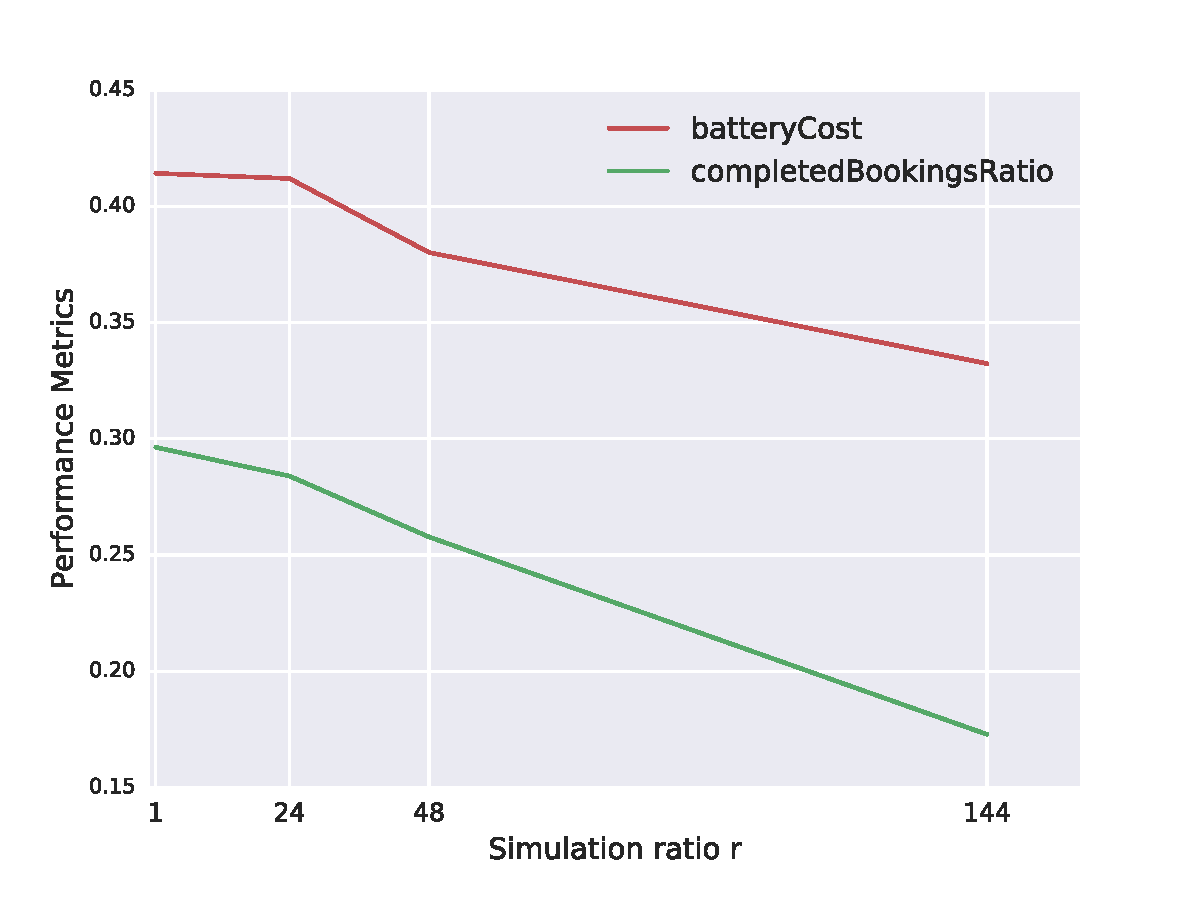
\includegraphics[scale=0.7]{./images/stability.pdf}
\caption{Performance metrics at growing simulation ratio $r$.}
\label{fig:stability}
\end{figure}

\subsubsection{Vehicles' Actor Speed} As explained in section \ref{simvehicles} the actors simulating the vehicles update their state (position and battery level) every 1000/$rate$ milliseconds. If $rate$ is too high the actor system end up with too many unhandled messages. On the other hand, if $rate$ is too small the vehicles skip stops. A good compromise is achieved with a $rate$ of 3.

\subsubsection{Time Consistency Between Applications} We need to assess if the Core-Engine application receives the bookings at the same time the World-Simulator application sends the booking through a REST API. In fact, there might be some delay as the World-Simulator checks every second if it needs to send bookings, so if there is a real-time delay of one second it can increase proportionally to the simulation ratio $r$. We compare the time at which the booking is supposed to be sent $simTime^{b}$ from the World-Simulator to the reported time in the logs from the Reporting application which populates its database at $sampleInterval$ of one second. We obtain that on average the difference is of 5 seconds and it never exceeds 55 seconds. It is totally acceptable as we run simulations over one day. Moreover, the vehicles' logs we get from the Reporting application are at regular $interval$ of 10 seconds.

\begin{table}
\makebox[\textwidth][c]{
  \centering
\begin{tabular}{| l | l |}
  \hline			
  Simulation Parameter & Value \\
\hline	  
  $r$ & 24\\
  $rate$ & 3 \\
  $interval$ & 10 seconds \\
  $sampleInterval$ & 1 second \\  
  \hline  
\end{tabular}
}
\caption{Simulation framework's parameters used.}
\label{table:simparametersused}
\end{table}

\subsection{Scenario Settings}
In order to compare different scheduling strategies and different scenarios, we run all scenarios with the same type of vehicles on the same fixed line. In what follows all the parameters used for the simulation are detailed.
\subsubsection{Vehicles}\label{vparam}
Each vehicle $v$ composing the fleet $V$ has a capacity $c^{v}$ = 10. The battery level varies from 0 to $q^{v} = 1$. The battery discharges, proportionally to its speed $s$ given in miles per hour, at each actor step of simulated duration $\delta = r * 0.33$ seconds by:
\begin{equation} \label{vehicleequation}
((0.0261905 * s^{2} + 1.70238 * s + 95.3571) * s) * \Delta * \beta^{v}
\end{equation}
and similarly it recharges by $ \Delta * \alpha^{v}$.
The homogeneous fleet has ratios $\alpha$ and $\beta$ set to 1 unless stated otherwise. As explained in section \ref{schedule}, vehicles finish their missions and go to charge if their battery level is under $minBatt$ = 0.3. Vehicles go at constant speed of 12.4 miles per hour as in cities with the current shuttle technologies and road settings it is not possible for them to go faster.
\subsubsection{Graph}
The fixed line is situated in Mountain View, California, with 32 stops situated at strategical points on the loop based on the types of area (accommodations, shopping centres industry, etc.). In current running autonomous transportation infrastructure, like for example in Sion for the project SmartShuttle, two vehicles are running on a fixed line and there is one depot where they can recharge. Currently it is reasonable to assume that all charging stations are centred at one place on the loop. We set therefore ten charging stations in the same area. The length TODO of the loop is of ... km.  

\begin{figure}
  \centering
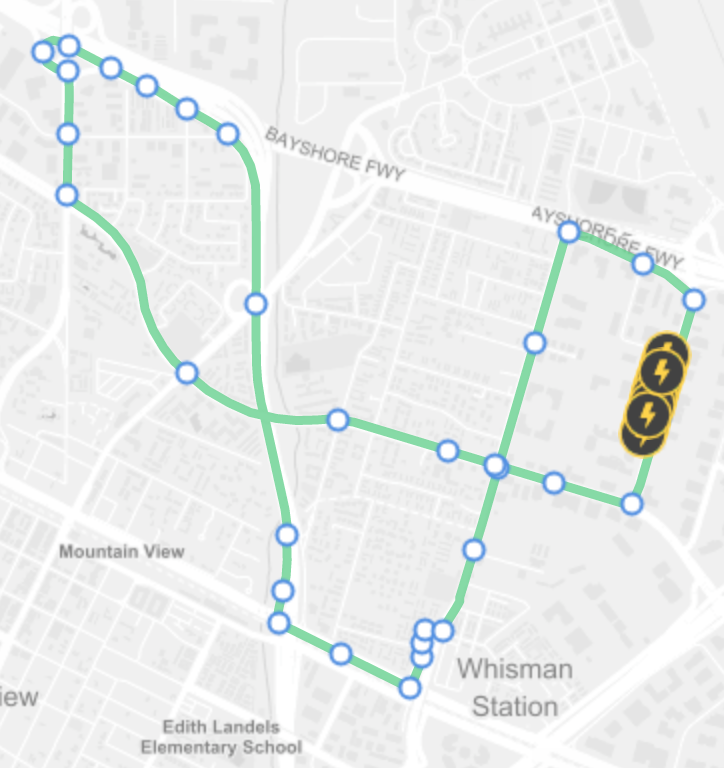
\includegraphics[scale=0.5]{./images/graph}
\caption{Fixed loop with 32 stops and 10 battery stations in the same area.}
\label{graph}
\end{figure}


\subsubsection{Simulated Demand}\label{simdem}
The goal of the simulations is to send realistic bookings in this specific loop over the scheduling horizon of one day in order to get meaningful metrics. As there is no available information of the demand distribution on this specific loop, other data can be analysed and realistic bookings can be extrapolated from it. The simulated demand is estimated analysing traffic information data of the area of study provided by HERE Maps. This data set provides real-time traffic flow tags for the main road segments in the USA. There is for example the free-flow (maximum speed allowed) over the average speed at each minute of the day for each segment as well as the estimated number of vehicles. 20\% of the total number of vehicles is considered as public transport. The data over one week from Monday to Friday is selected for analysis. Generalized additive model is used to predict the number of vehicles for every minute at each edge of the graph. The change in number of vehicles between each segment is recorded in order to estimate the number of pick-up (when it increases) and drop-off (when it decreases). In order to simulate bookings from one of the 32 stations to an other station, the correlation matrix of the number of vehicles between the segments is used with a multinomial distribution with weights of the zoning area (residential, industrial or office) to generate bookings from one station to an other for a week-day starting at midnight. The output is a list of 584 bookings with varying number of passengers $1 \leq n^{b} \leq 5$. The number of bookings generated every hour of the scheduling horizon of one day is represented in Figure \ref{fig:demand}.

\begin{figure} 
  \centering
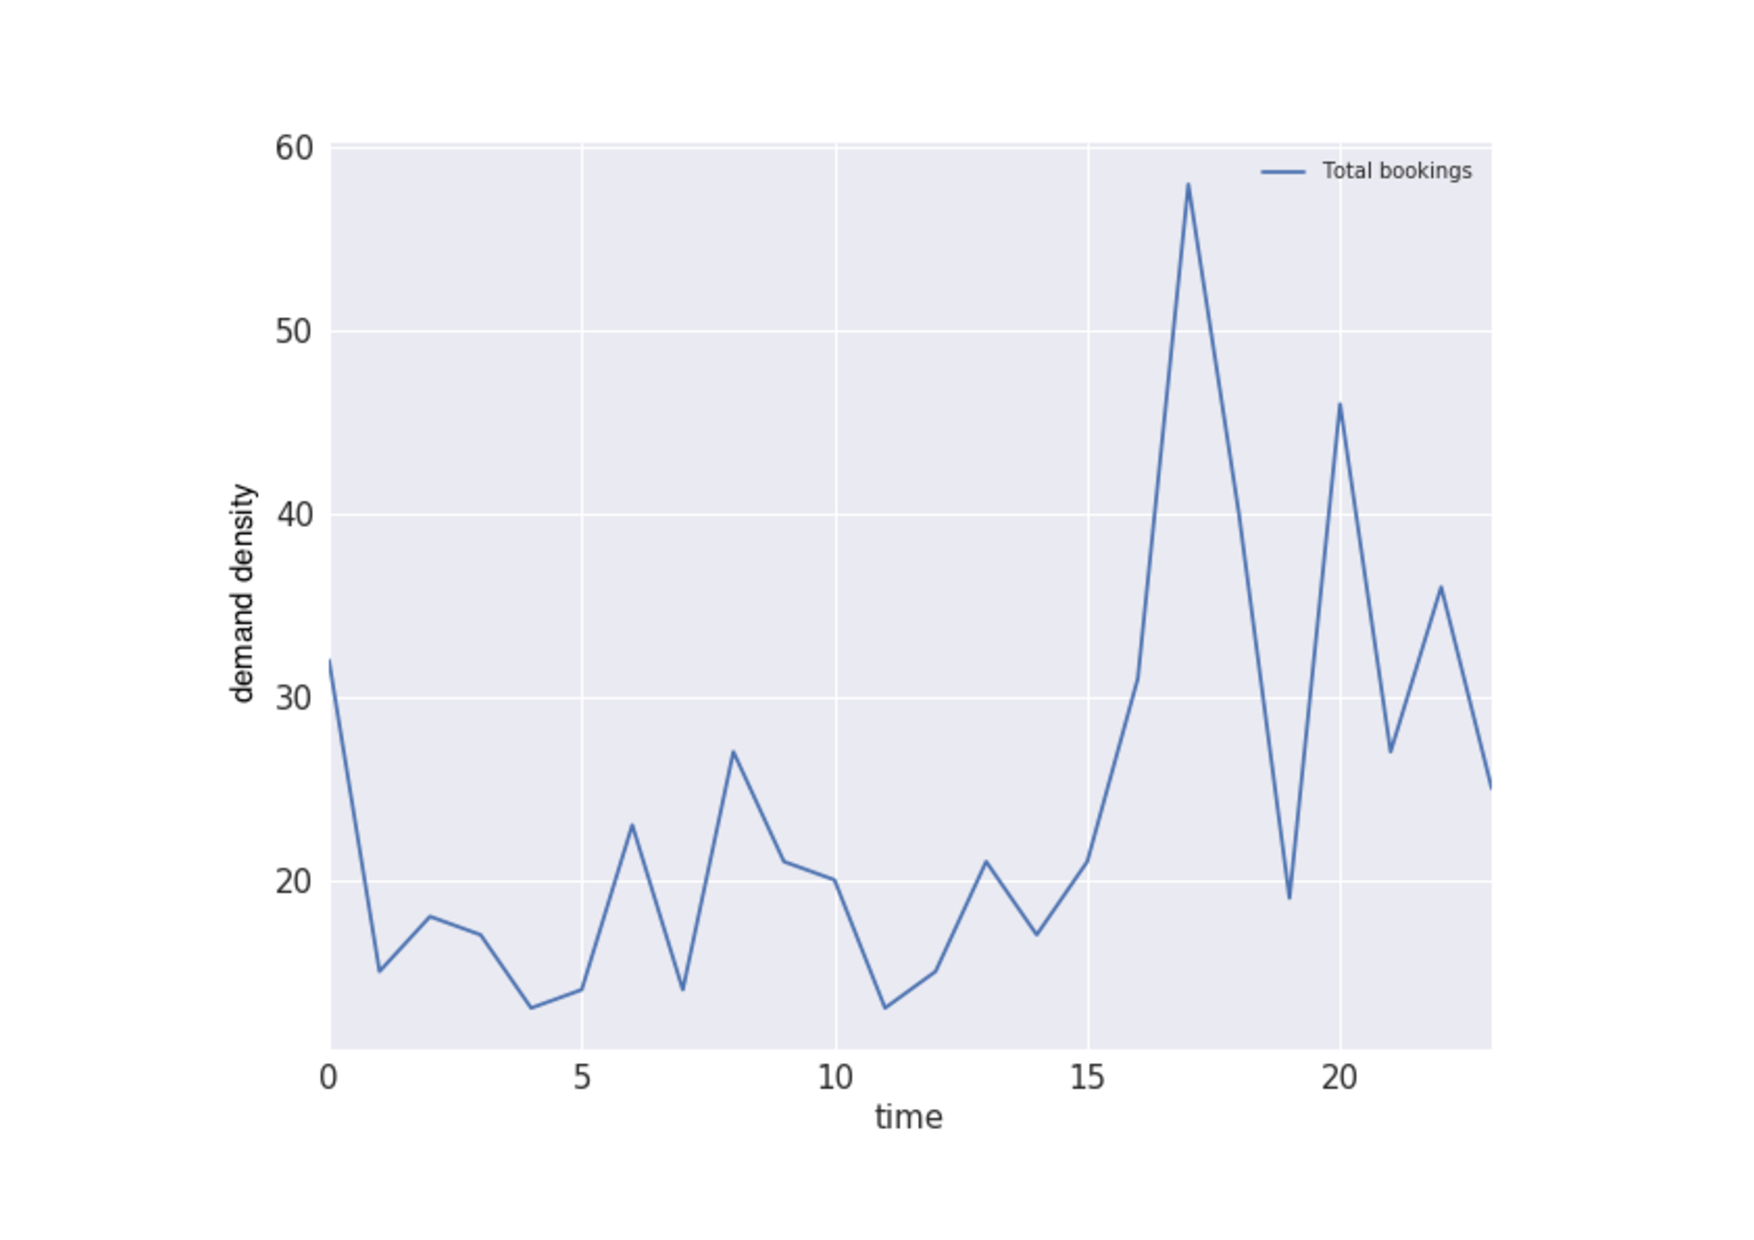
\includegraphics[scale=0.5]{./images/demand.pdf}
\caption{Demand density $dem_{t^{*}}$ at each hour of a week-day.}
\label{fig:demand}
\end{figure}

\subsection{Headway Experiments}\label{hwexperiments}
As explained in section \ref{hw}, we adopt a strategy involving the vehicles to wait at mandatory stations during an adaptive stopping time based on the distance to the next vehicle on the loop. In order to analyse what is the impact on the transportation service, we compare the output of the simulation metrics when running with the dynamic waiting strategy or without. We analyse the results of the simulations with only mandatory stops or with only optional stops. The following strategies are therefore simulated:
\begin{enumerate}
\setlength\itemsep{1pt}
\item \textbf{Constant $wait_t^{v}$}: every time a vehicle arrives at a station it waits 20 seconds, in other words $default= 20''$ and $ratio$ is always equal to 1. 
\item \textbf{Adaptive $wait_t^{v}$}: when a vehicle arrives at a station it waits $wait_t^{v} = default * ratio$, with $default = 20''$ and $ratio$ computed as explained in section \ref{hw}. The minimum waiting time $waitMin$ is $2''$ and the maximum waiting time $waitMax$ is $10'$.
\begin{enumerate}
\item \textbf{Mandatory stops} $\forall s \in S: M^{s} = 1$. The adaptive waiting time is computed each time a vehicle arrives at a station.
\item \textbf{Optional stops} $\forall s \in S: M^{s} = 0$. When a vehicle arrives at a station if it does not need to stop for passengers it can skip the stop: $wait_t^{v} = 0$.
\end{enumerate}
\end{enumerate}
We run the simulations over a scheduling horizon $H$ of one day, with the simulated bookings obtained as explained in section \ref{simdem}. The fleet is composed of 8 homogeneous vehicles always active, with the characteristics enumerated in section \ref{vparam}. 

\begin{figure}
  \centering
\begin{subfigure}[b]{0.435\textwidth}
  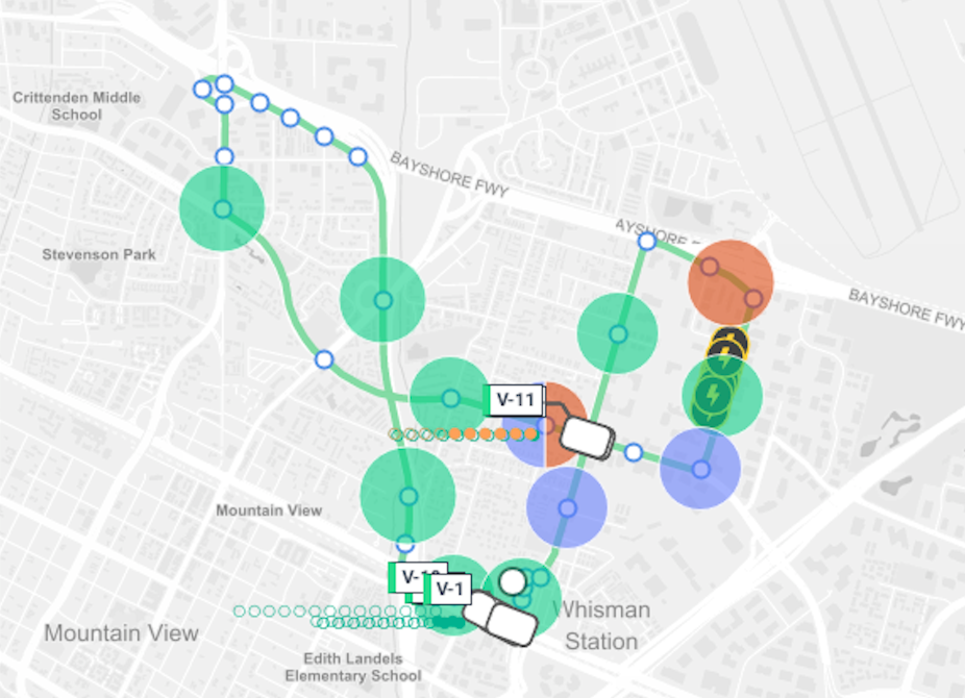
\includegraphics[width=\linewidth]{./images/busbunching.pdf}
  \caption{Constant $wait_t^{v}$}
  \label{busbunching}
\end{subfigure}
\begin{subfigure}[b]{0.4\textwidth}
  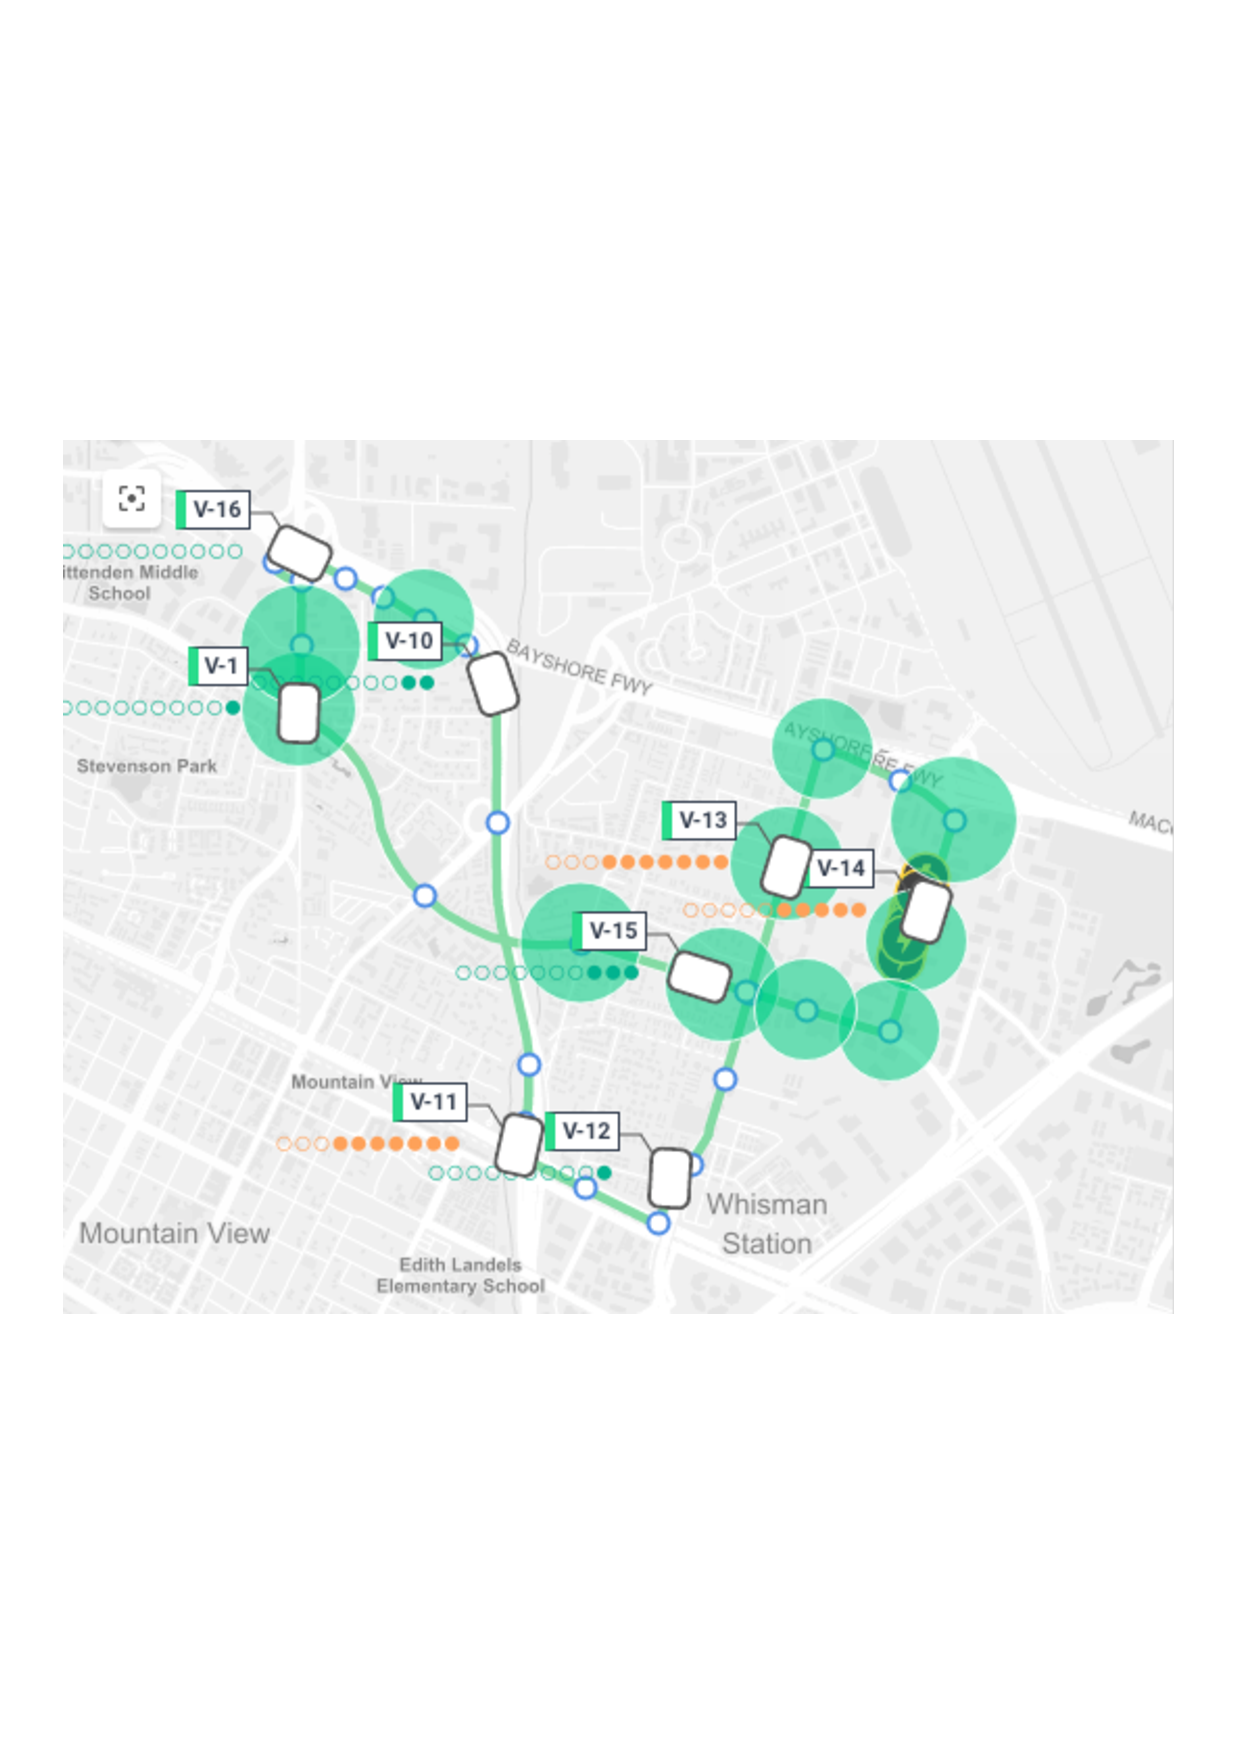
\includegraphics[width=\linewidth]{./images/spread.pdf}
  \caption{Adaptive $wait_t^{v}$, mand. stops}
  \label{adaptive}
\end{subfigure}
\begin{subfigure}[b]{0.4\textwidth}
  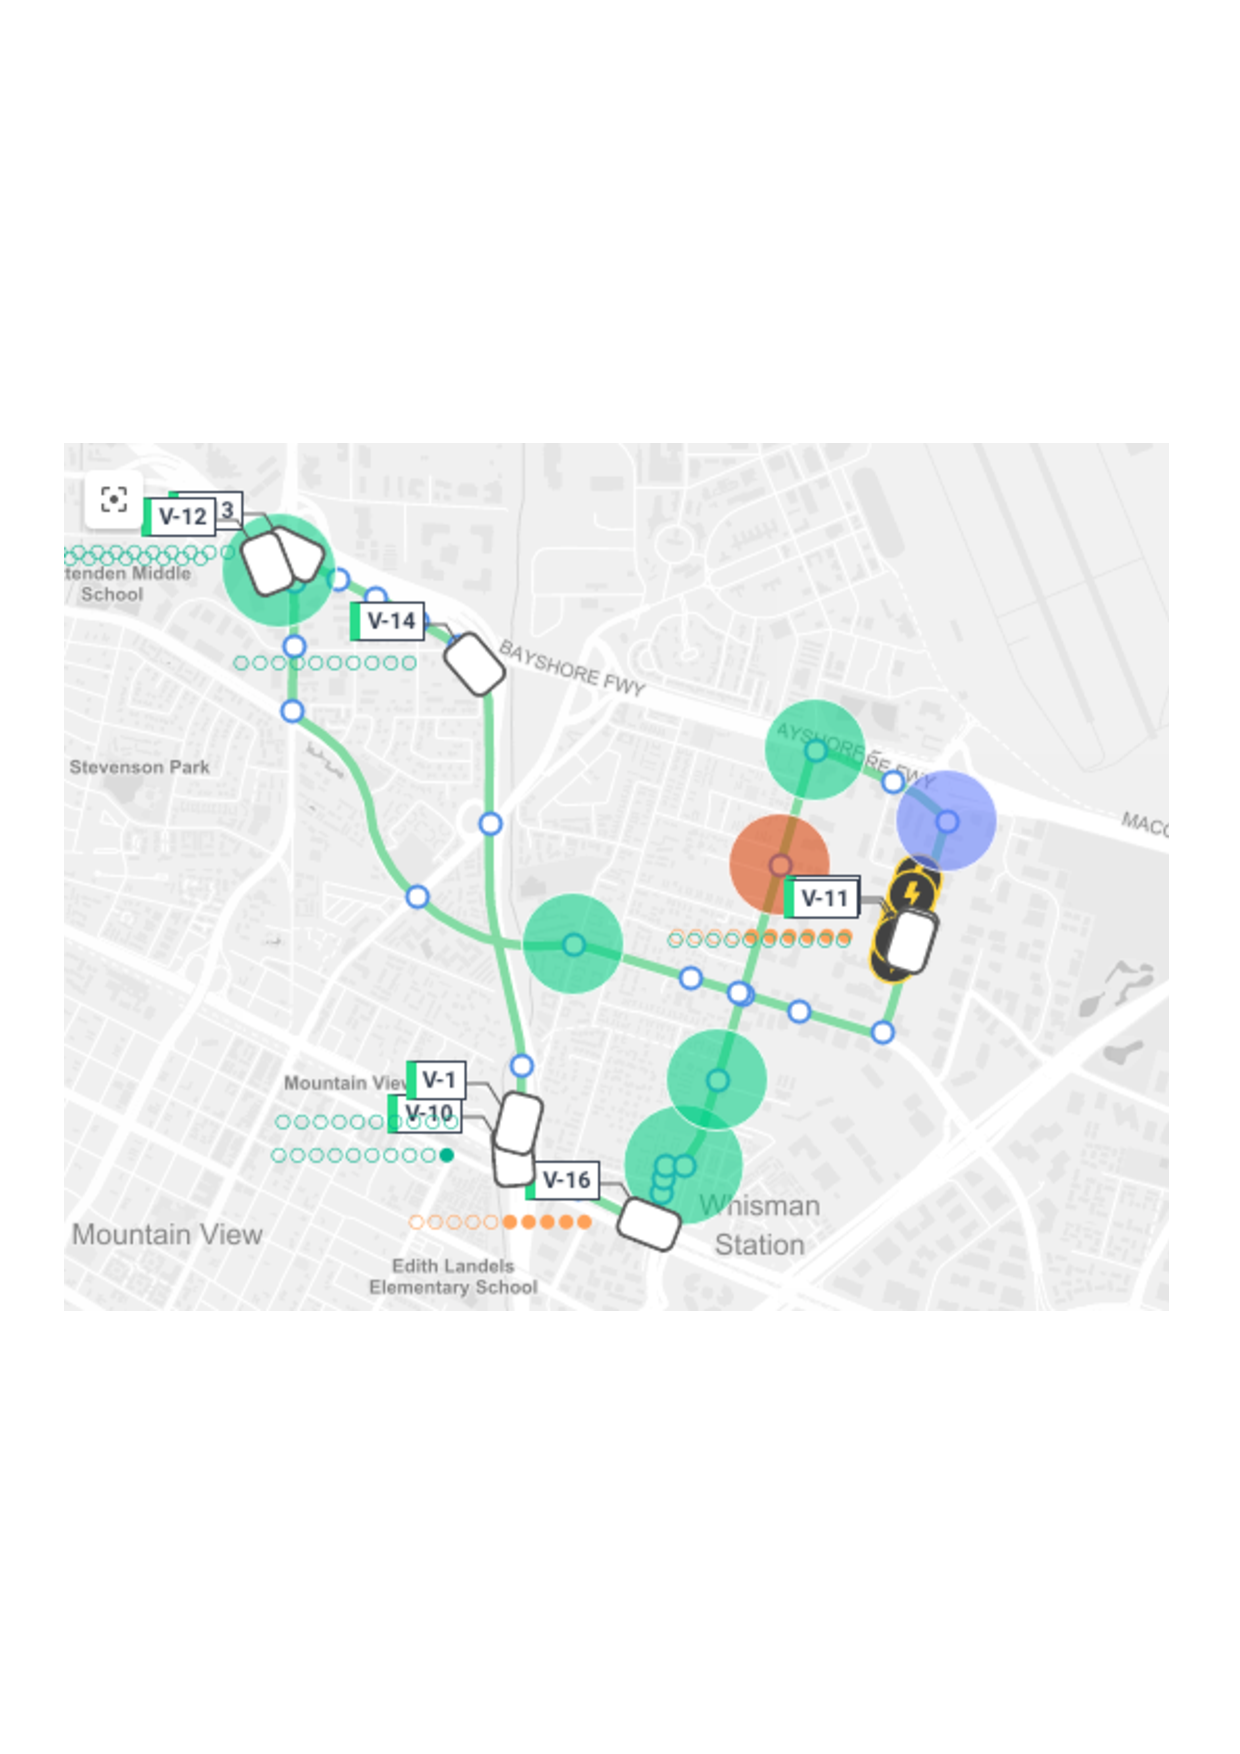
\includegraphics[width=\linewidth]{./images/optionalstopsgroup.pdf}
  \caption{Adaptive $wait_t^{v}$, optional stops}
  \label{skip}
\end{subfigure}

\label{simustate}
\caption{Vehicles' positions on the fixed line at $simTime$ = 6:00am illustrating the space between vehicles.}
\end{figure}

The state of the fixed line at the same simulated time ($simTime$ = 6:00am) is shown in Figure \ref{simustate}. The green dots stand for the pick-up station of the bookings which are being processed with the drop-off stations in purple. The red dots are the customers which have not been picked up yet. As you can observe in Figure \ref{busbunching}, when there is no particular strategy adopted to maintain the ideal distance between the vehicles, they end up in two distinct bus convoys of four shuttles each. It happens because the preceding shuttles can not take over the one picking up and dropping the passengers in the front. This phenomenon is illustrated in Figure \ref{constanthw}: the average occupancy is higher over the entire day especially for one vehicle. In Figure \ref{adaptiveload} we can see that adapting the stopping time at each station works well for maintaining an ideal distance between the shuttles. Until the end of the simulation no convoy is formed and the $loadFactor$ per vehicle is stable. In fact, the $loadFactorStability$ is 0.003 as opposed to 0.034 for the constant stopping time strategy. If we allow shuttles to skip stations, the distance between them is not really stable as the distance is not regulated every time they reach a station, but the $loadFactorStability =  0.006$ is still low.  The percentage change of the performance metrics of adaptive waiting time strategy relative to the constant stopping time is represented in Figure \ref{hwcompare}. We can see that the battery consumption increases a lot if stops can be skipped as vehicles are never forced to stop when the demand is low. Moreover, vehicles wait on average $35''$ if the stops are mandatory and $25''$ if they are optional. The $avgWaitingTime$ is 10 minutes if all stops are mandatory and 5 minutes if stops can be skipped. This has a substantial impact on the level of service offered to the passengers. However, less bookings are satisfied at the end of the day with only optional stops. This is probably due to the fact that vehicles do not always maintain the ideal distance between them. 

\begin{figure}
  \centering
\begin{subfigure}[b]{0.445\textwidth}
  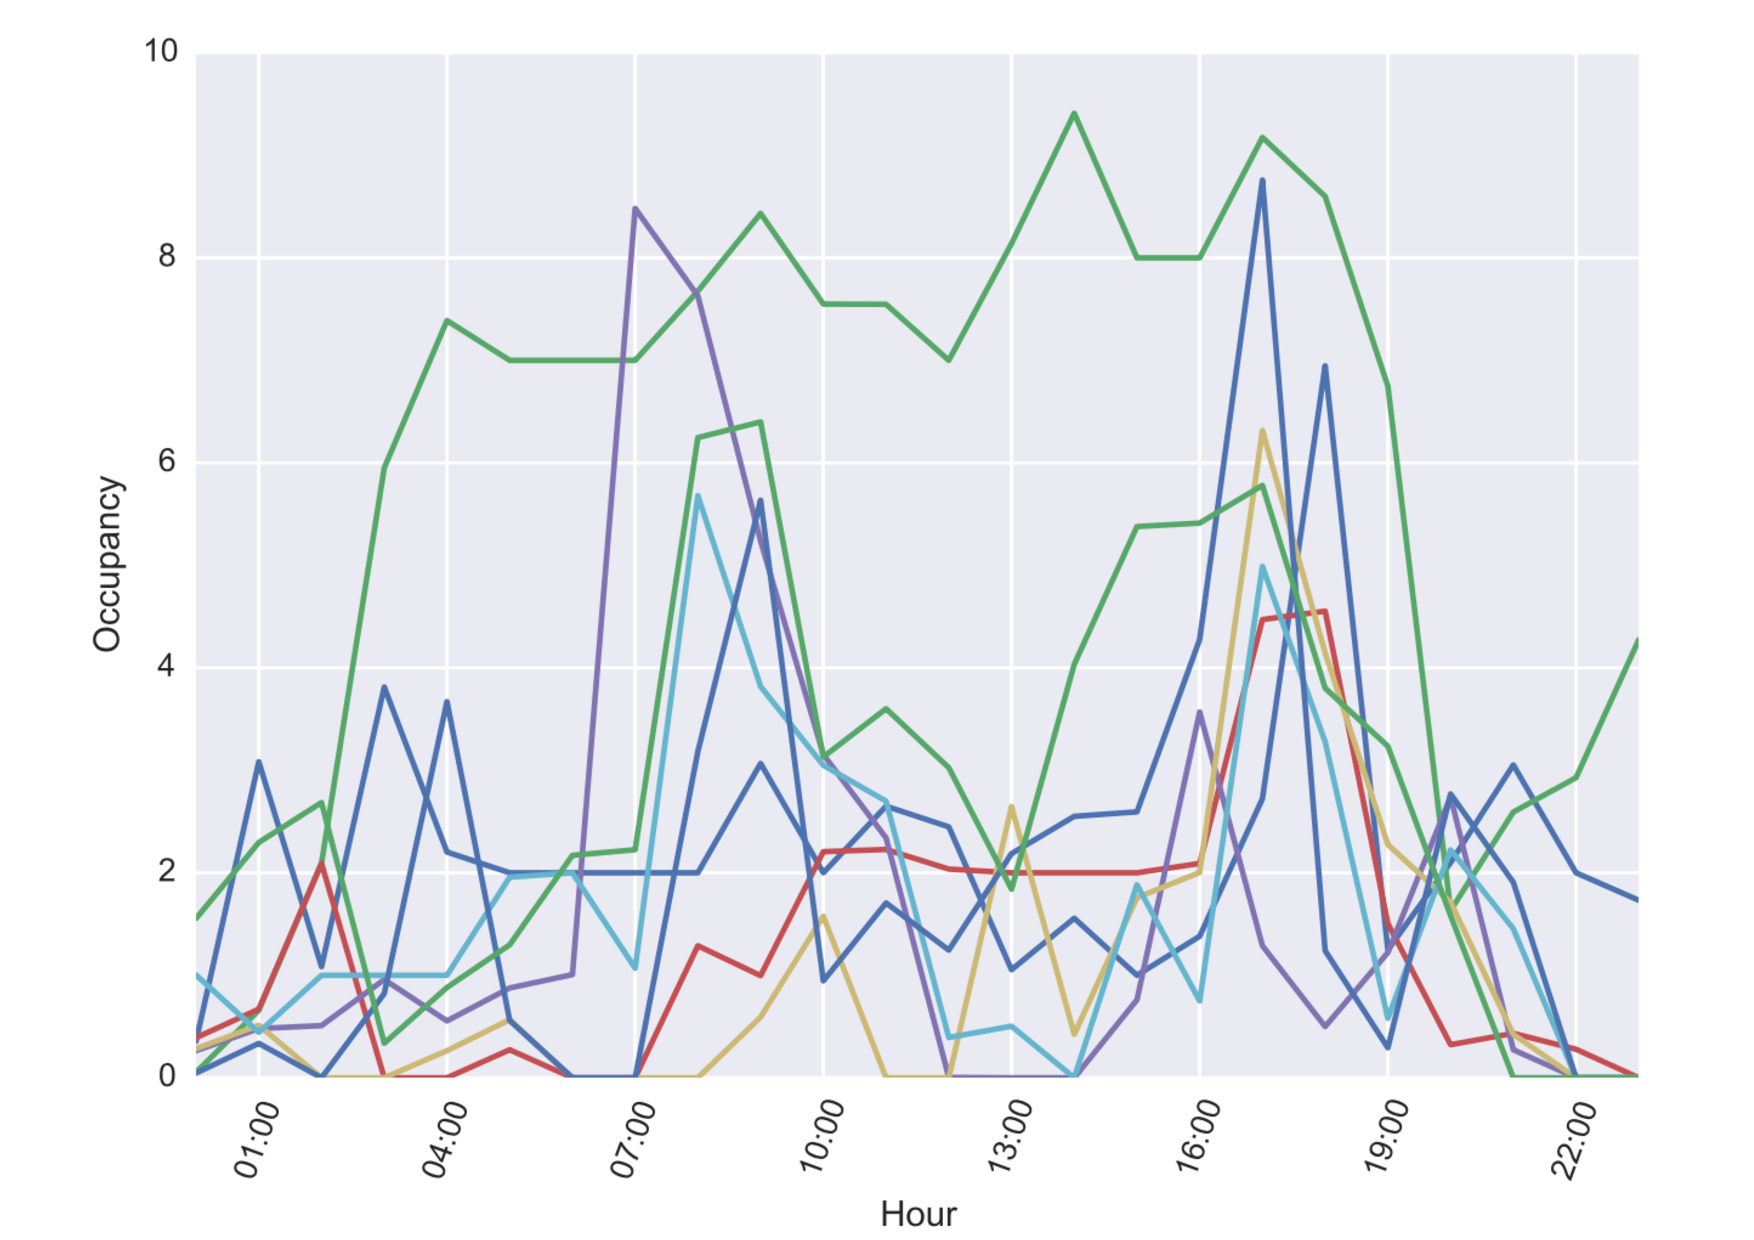
\includegraphics[width=\linewidth]{./images/constanthw.png}
  \caption{Constant $wait_t^{v}$}
  \label{constant}
\end{subfigure}
\begin{subfigure}[b]{0.42\textwidth}
  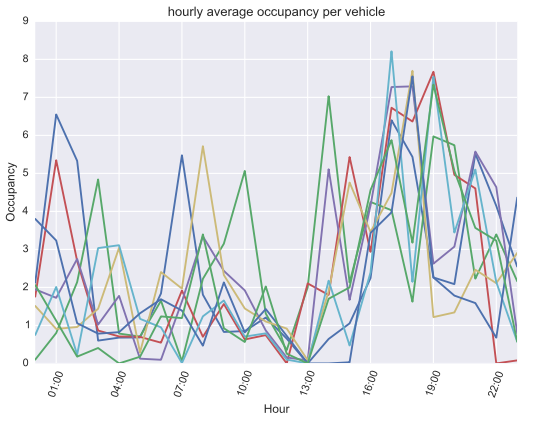
\includegraphics[width=\linewidth]{./images/hwmax10simu}
  \caption{Adaptive $wait_t^{v}$, mand. stops}
  \label{adaptiveload}
\end{subfigure}
\begin{subfigure}[b]{0.49\textwidth}
  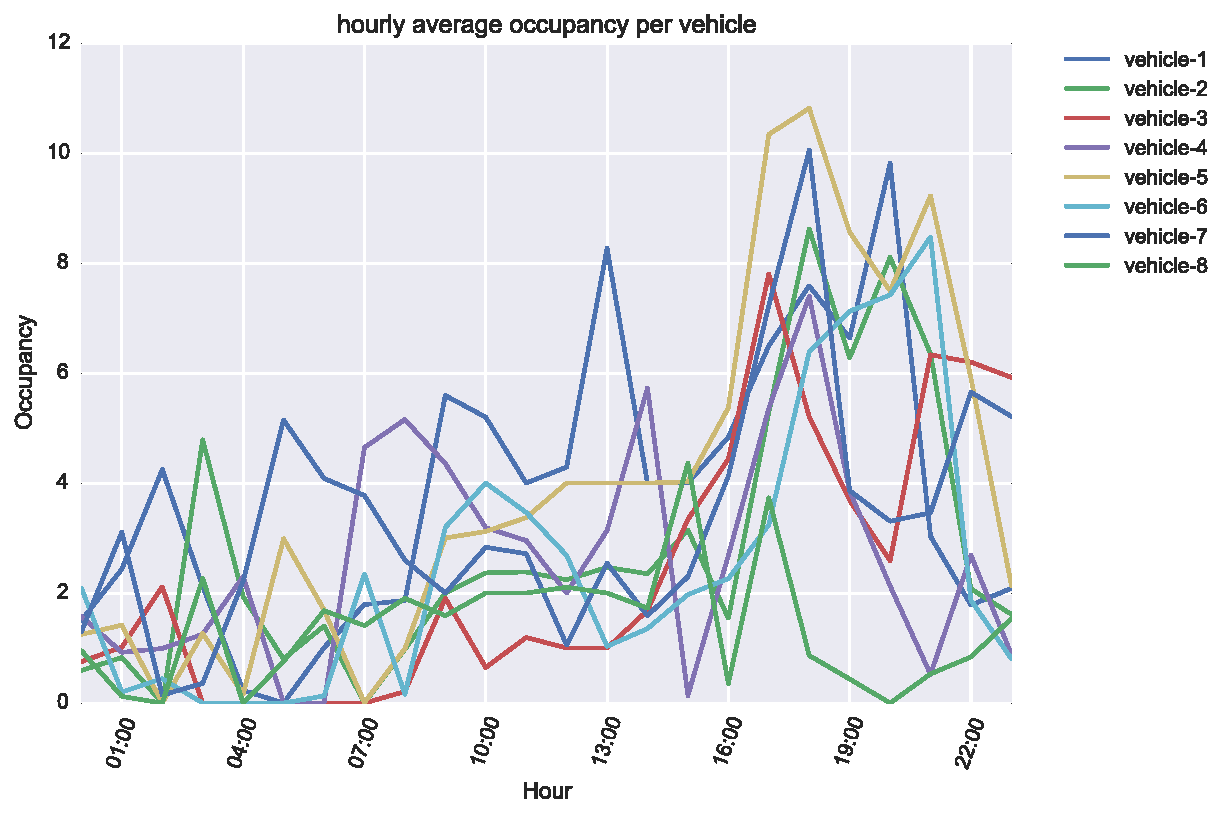
\includegraphics[width=\linewidth]{./images/optionalstops}
  \caption{Adaptive $wait_t^{v}$, optional stops}
  \label{skipload}
\end{subfigure}
\label{simuload}
\caption{Average occupancy of each vehicle at each hour of the day.}
\end{figure}

\begin{figure}
  \centering
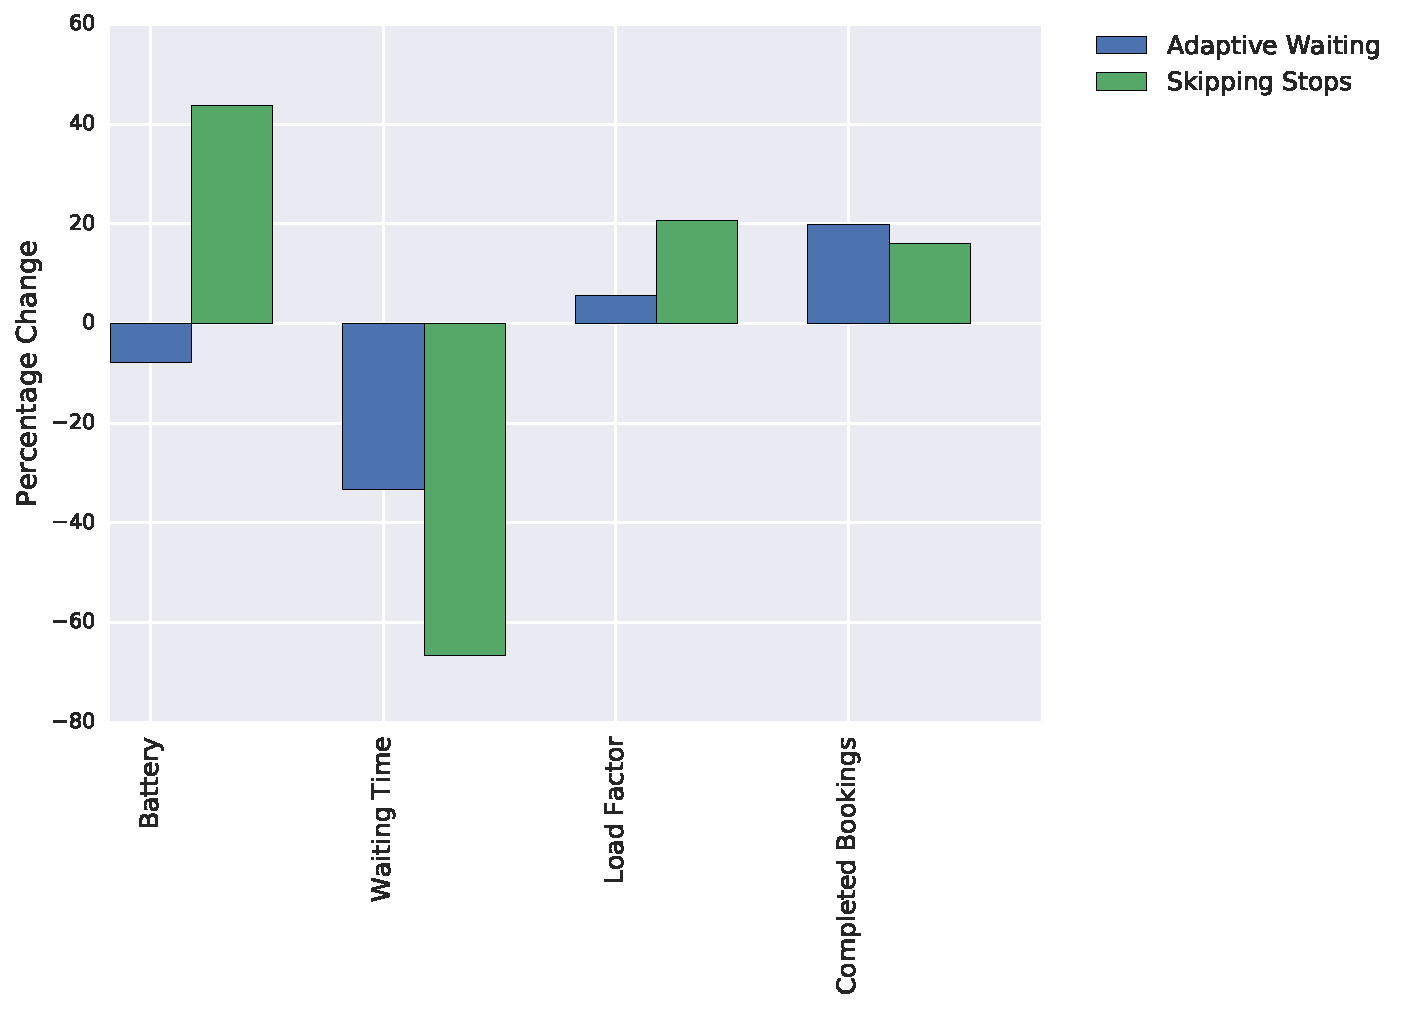
\includegraphics[scale=0.48]{./images/headwayCompare.pdf}
\caption{Percentage change of the adaptive waiting strategies' performance metrics relative to the constant stopping time strategy.}
\label{hwcompare}
\end{figure}

\subsection{Dynamic Fleet Size Experiments}
In what follows we present the several stages conducted in our experimental analysis TODO write intro 
say that we use adaptive wait with mandatory stops
\subsubsection{Generating Data}\label{data}
As explained in section \ref{dynamic}, in order to get insights about the impact of the number of vehicles with varying demand density on the performance metrics we need to run several simulations and gather all the data. As simulations are time-consuming, we need to choose which sampling $D$ of demand density we want to simulate. Based on the demand density frequency over the day which is plotted in Figure \ref{demfreq}, we run simulations for $dem \in D = \{13, 15, 21, 23, 25, 27, 31, 36, 40, 46, 58\}$. For each demand density we generate a list of bookings at fixed interval $1h / dem$. Simulations are then run over one hour with varying the fleet size from $V^{-}=$2 vehicles to $V^{+}=$10 vehicles. For each simulation of varying demand density and fleet size the performance metrics are recorded. As the simulations are subject to some perturbation due to the accelerated time, we clean the data by replacing the values lower than the 5$^{th}$ quantiles and higher than the 95$^{th}$ quantiles. Figure \ref{values} displays all the data collected after the simulations.
TODO: replace with values after cleaning

\begin{figure} 
  \centering

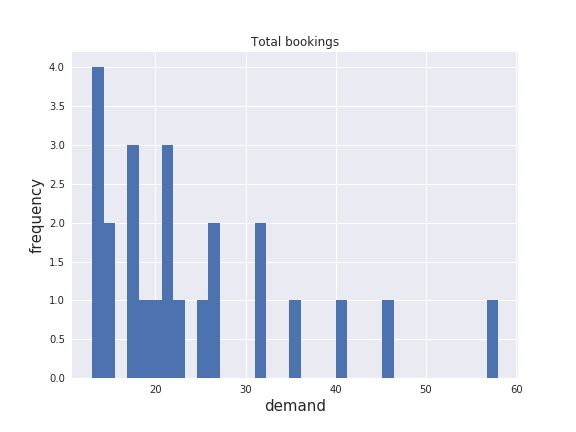
\includegraphics[scale=0.6]{./images/demand_freq.png}
  \caption{Demand density frequency over the simulated day.}
\label{demfreq}
\end{figure}


\tiny{
\csvreader[
  longtable=lllll,
  table head=   \label{values}\\\hline
    \toprule\bfseries dem &\bfseries |V|&\bfseries batteryCost &\bfseries avgWaitingTime&\bfseries completedBookingsRatio\\ \midrule\endhead
    \bottomrule\endfoot,
  late after line=\\,
  late after last line=\\\bottomrule,
  before reading={\catcode`\#=12},after reading={\catcode`\#=6},
  table foot = \caption{Performance metrics obtained after running simulation for each demand density and fleet size combination.}
]{values2.csv}{1=\a,2=\b,3=\c,4=\d,5=\e}{\a & \b & \c & \d & \e}
}


\normalsize
\subsubsection{Fleet Size's Impact On Performance Metrics}\label{impact}
In this section we present the analysis of the simulations' output metrics in order to describe the relationships between the fleet size and the performance measures and how it varies with the demand density.

\paragraph{Average Performance Metrics} 
In Figure \ref{averages} the performance metrics' averages over all demand densities $dem \in D$ at growing fleet size are represented. As expected, the $batteryCost$ and the $completedBookingsRatio$ increase proportionally to the fleet size whilst the $avgWaitingTime$ and the $averageLoadFactor$ decrease. The percentage changes of the different costs are enumerated in table \ref{averageschange}. As you can see, the average waiting time decreases from 16.8 minutes to 3.18 minutes which is really relevant to the quality of the transportation service. However, if it is costly to run the vehicles the change in battery consumption is weighty when the fleet size increases and the vehicles are not used efficiently as the $avgLoadFactor$ is low.

\begin{figure}
  \centering
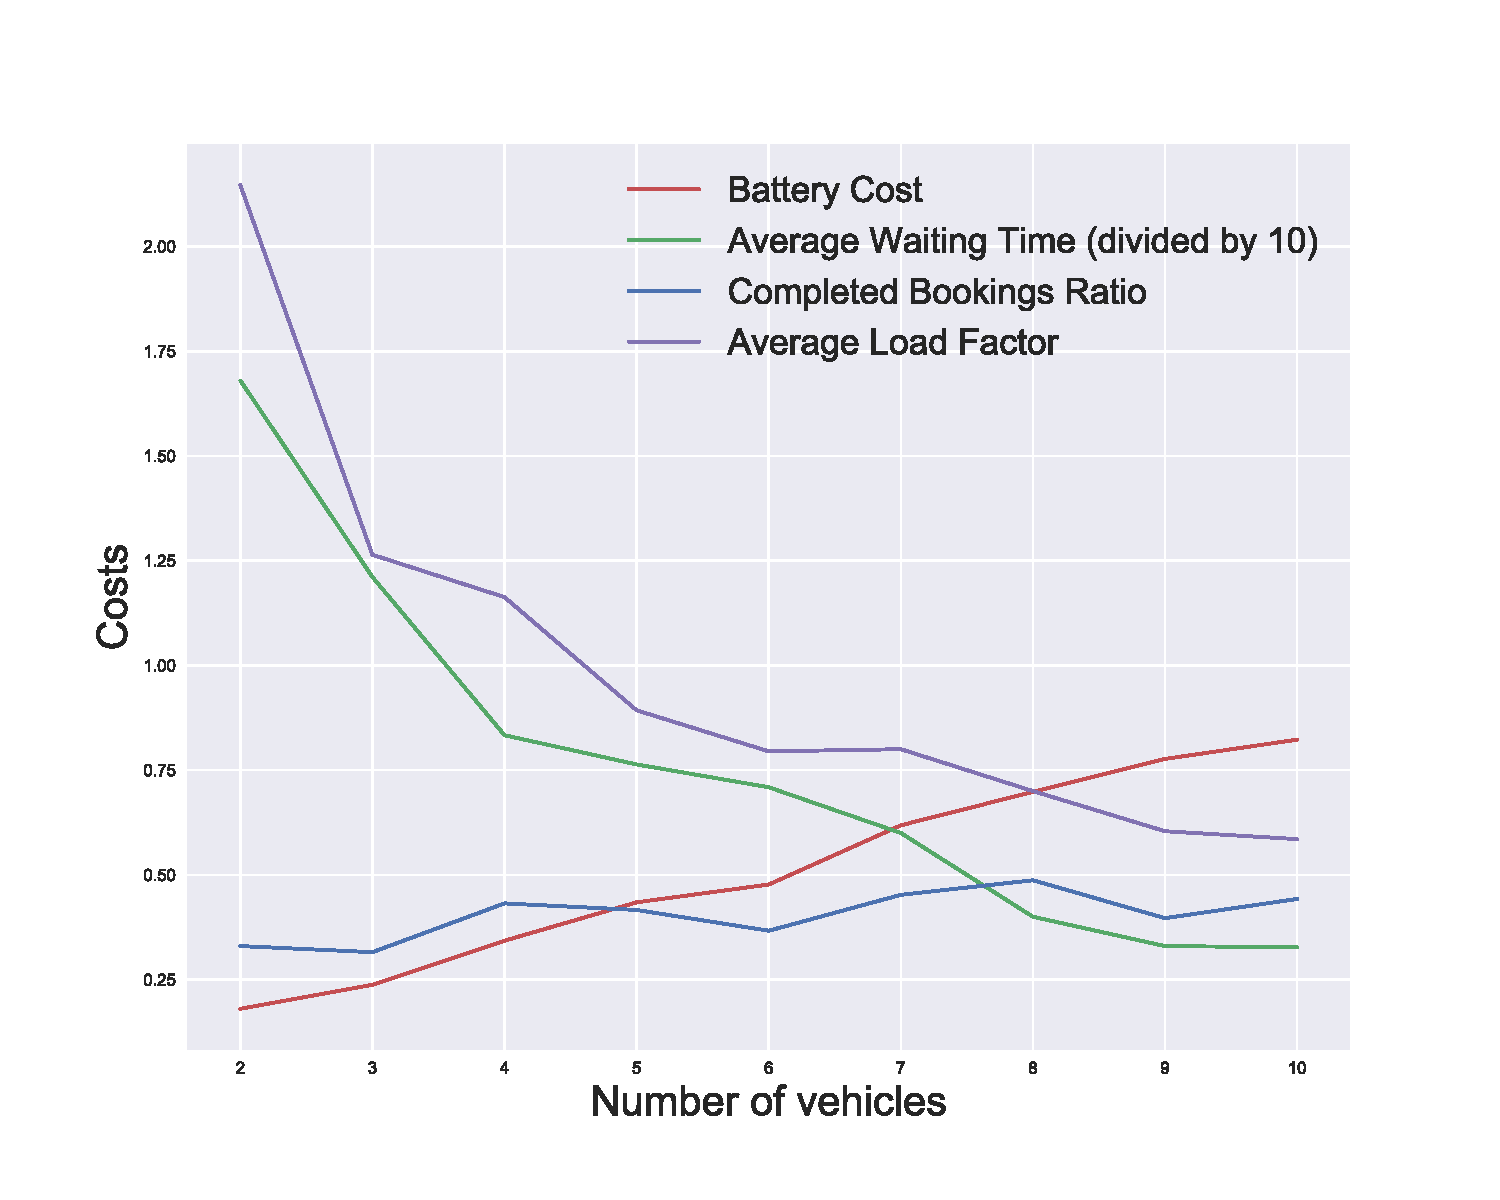
\includegraphics[scale=0.5]{./images/vehicleimpact.pdf}
  \caption{Performance metrics averages over all demand densities $dem \in D$ at growing fleet size.}
\label{averages}
\end{figure}


\begin{table}[h]
\caption{Percentage change between of average performance metrics when running simulations with two and ten vehicles.}
\center
    \begin{tabular}{|l|r|l|r|}
      \toprule
    & $|V|$=2 & $|V|$=10 & Percentage Change\\
    \midrule
    $batteryCost$ & 0.17 & 0.84 & 394\%\\
    $avgWaitingTime$ & 16.8' & 3.18' & -80\% \\
    $avgLoadFactor$ & 0.21 & 0.06 & -71\% \\
    $completedBookingsRatio$ & 0.33 & 0.44 & 33\% \\
    $avgJourneyTime$ & 27' & 20' & -26\% \\
    \midrule
    \end{tabular}
    \label{averageschange}
  \end{table}
  
\paragraph{Demand Density and the Fleet Size's Impact on Performance Metrics}
For each of the three measures $batteryCost$, $avgWaitingTime$ and $completedBookingsRatio$ we analyse the growth of the costs regarding the fleet size and the demand density:
\begin{itemize}
\item $batteryCost$: We suppose from Figure \ref{batterycost} that the battery consumption grows linearly regarding the number of vehicles and that it is not dependent on the demand density. In fact, the correlation coefficient between $batteryCost$ and $|V|$ is 0.9 whilst between $batteryCost$ and $dem$ it is equal to -0.09. Moreover, we perform a linear regression with the explanatory factor being the fleet size $|V|$ and the dependent variable the $batteryCost$. We obtain a coefficient of determination $R^{2} = 0.88$, which means that it explains 88\% of the variance. We conclude that the energy cost grows linearly to the number of vehicles active on the line. 

\item $avgWaitingTime$: From Figure \ref{wtcost} we can see that the waiting time is not only dependent on the fleet size but on the demand density as well. In fact, the correlation between $avgWaitingTime$ and $|V|$ is -0.48 and with $dem$ it is equal to 0.24. We run therefore a linear regression with the explanatory factors being the fleet size $|V|$ and the demand density $dem$ and we obtain $R^{2}$ = 0.4. However, the average waiting time varies from different ranges between the different group of same demand density, affecting the regression which will fit a line on the average of those $avgWaitingTime$ values. In order to overcome this multicollinearity problem, we can add a dummy variable for each but one group of 9 instances (fleet size being between 2 and 10), a group being the instances with the same demand density $dem \in D$. We perform a linear regression with the predictors being $dem$, $|V|$ and the dummy variables and we obtain a better coefficient of determination $R^{2} = 0.53$. The normal probability plot of the linear regression which looks fairly straight is shown in Figure \ref{probaplot}. However, we suppose from Figure \ref{averages} that an exponential function could fit better the observed $avgWaitingTime$. We run a non-linear regression, fitting the $avgWaitingTime$ to the exponential function $a * e^{[b_{1},...,b_{|D|+2}]*[dem,|V|,dummyVar]}+c$ with the demand density, the fleet size and the dummy variables as predictors. We compare the residual sum of squares $RSS$ of both models on our datapoints. For the linear model we obtain a $RSS$ =   1709 and for the exponential model $RSS = 1331$. The $RSS$ of the exponential model is 22\% smaller than the $RSS$ of the linear model. The $avgWaitingTime$ decreases therefore exponentially as the number of vehicles increase.
TODO put plot of the fit
\begin{figure}[h] 
  \centering
  \caption{Linear regression residuals' probability plot for the function fit of the $avgWaitingTime$}
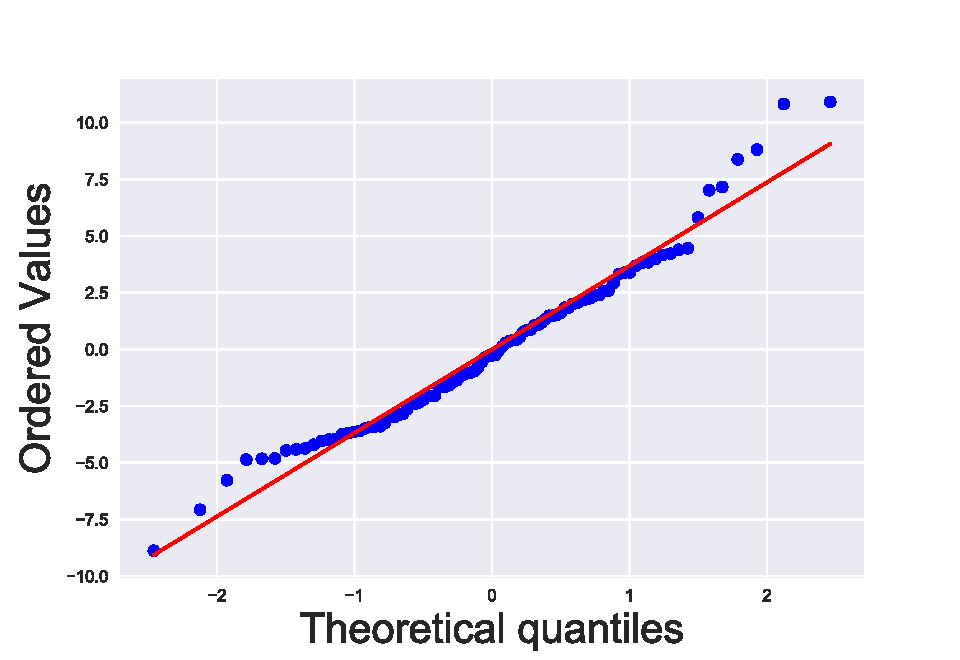
\includegraphics[scale=0.4]{./images/probaplot.pdf}
\label{probaplot}
\end{figure}

\item $completedBookingsRatio$: As opposed to the $batteryCost$ and $avgWaitingTime$ which have a higher correlation with the fleet size $|V|$ than the demand density $dem$, the $completedBookingsRatio$ has a correlation coefficient with the demand density (-0.39) which is more significant than with the fleet size (0.25). It is indeed normal as the ratio of completed bookings is higher if there are less bookings sent during the simulated hour. We run a linear regression with the demand density $dem$, the fleet size $|V|$ and the dummy variables as predictors and we obtain $R^{2} = 0.61$ and $RSS = 0.77$. If we fit the $completedBookingsRatio$ to the exponential function we obtain $RSS = 0.71$.

\end{itemize}

\begin{figure}
\caption{Simulations' output metrics with respect to the fleet size $|V|$ (x-axis) and the demand density $dem$ (y-axis)}
  \centering
\begin{subfigure}[b]{0.452\textwidth}
  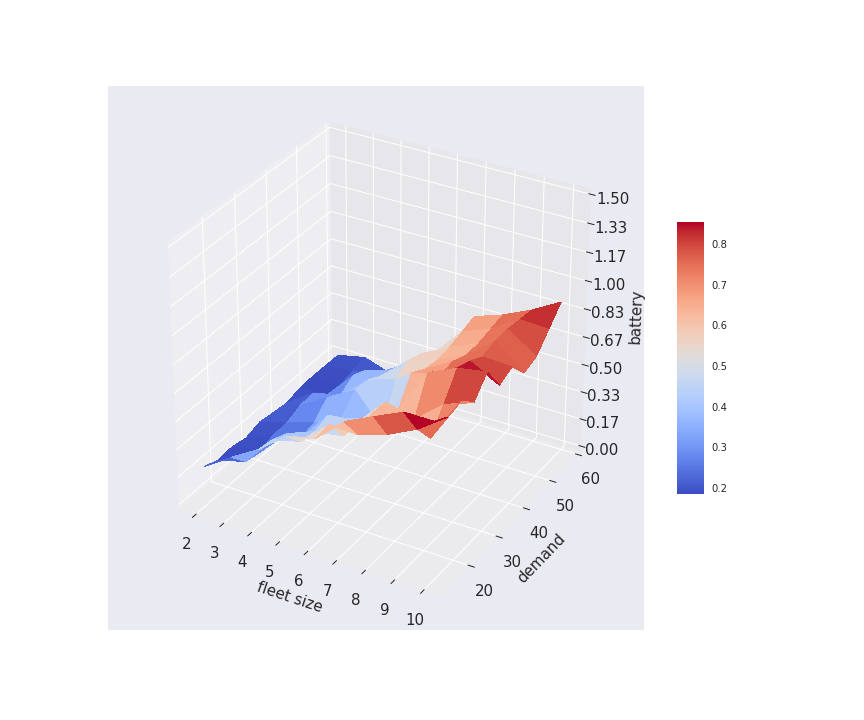
\includegraphics[width=\linewidth]{./images/battery.png}
  \caption{$batteryCost$}
  \label{batterycost}
\end{subfigure}
\begin{subfigure}[b]{0.45\textwidth}
  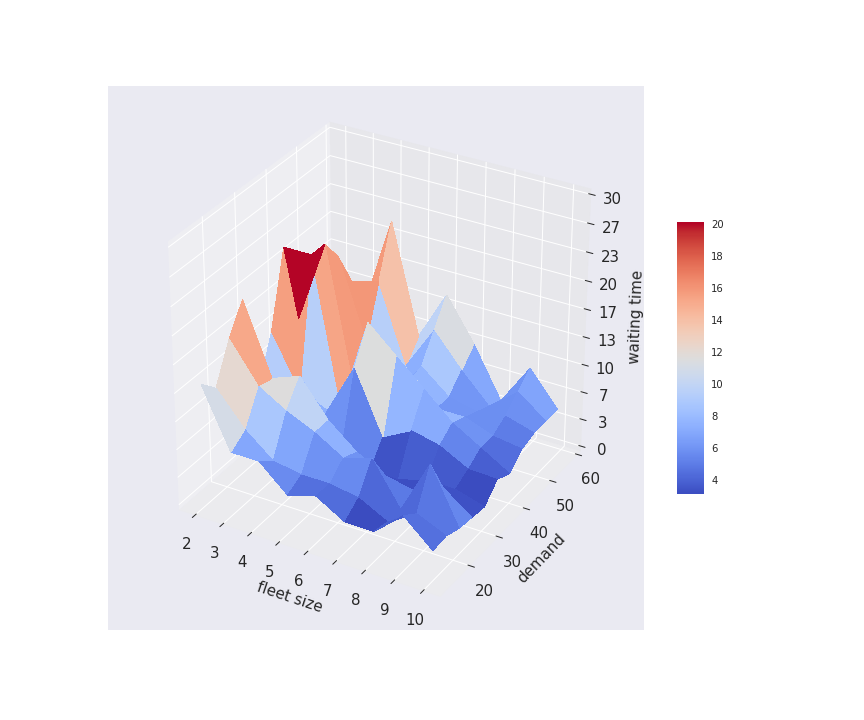
\includegraphics[width=\linewidth]{./images/waitingtime.png}
  \caption{$avgWaitingTime$}
  \label{wtcost}
\end{subfigure}
\begin{subfigure}[b]{0.458\textwidth}
  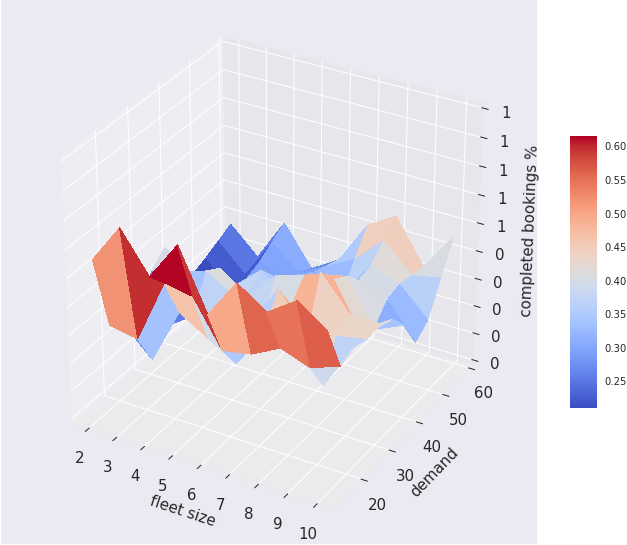
\includegraphics[width=\linewidth]{./images/completed.png}
  \caption{$completedBookingsRatio$}
  \label{cbr}
\end{subfigure}

\label{simustate}
\end{figure}


  \begin{table}
  \caption{Correlation coefficients between performance metrics and demand density and fleet size.}
  \vspace{-1.5em}
  \center
    \begin{tabular}{|l|r|r|}
     \toprule
    Correlation Coeff.& $dem$ & $|V|$ \\
    \midrule
    $batteryCost$ & -0.09 & 0.9\\
    $avgWaitingTime$ & 0.24 & -0.48\\
    $completedBookingsRatio$ & -0.39 & 0.25 \\
    $averageLoadFactor$ & 0.5 & -0.5\\
    \midrule
    \end{tabular}
    \label{correlation}
  \end{table}

\paragraph{Extreme Simulation Examples}
We to compare the fleet's behaviour and the performance metrics when the demand density is low to when it is high and how much the fleet size can actually improve the performance metrics in both cases. In Figure \ref{extremesimu}. In both cases the average waiting time is drastically reduced when the fleet is composed of ten vehicles as opposed to two vehicles. In fact, it decreases from 14 minutes to 3 minutes when the demand density is low $dem=13$ and from 12 minutes to 5 minutes for the highest demand density $dem = 58$. On the other hand, the $completedBookingsRatio$ increases by 13\% for $dem = 13$ (0.61 to 0.69) whilst it increases more substantially by 65\% for $dem = 58$. Moreover, we can observe that it is not efficient to have ten active vehicles when the demand is low as only four vehicles are used over the hour (see Figure \ref{dem13v10}). However, when the demand density is high the entire fleet is used over the hour (see Figure \ref{dem58v10}). This validates the idea that a larger fleet size is relevant mostly when the demand is high but that there is no need to use all the fleet size when the demand is lower.
\begin{figure}[]
\caption{Average occupancy of each vehicles at each minute of the simulated hour for the combinations of $V^{-}, V^{+}, dem^{-}$ and $dem^{+}$.}
%\makebox[\textwidth][c]{
  \centering
\begin{subfigure}[b]{0.48\textwidth}
  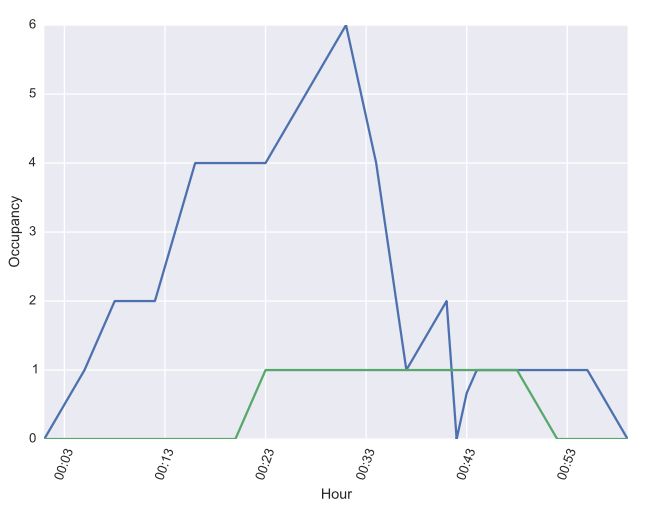
\includegraphics[width=\linewidth]{./images/dem13v2}
  \caption{$dem = 13, |V| = 2$\\ $avgWaitingTime = 14'$\\ $completedBookingsRatio = 0.61$ \\ $averageLoadFactor = 0.15$}
  \label{dem13v2}
\end{subfigure}
\begin{subfigure}[b]{0.48\textwidth}
  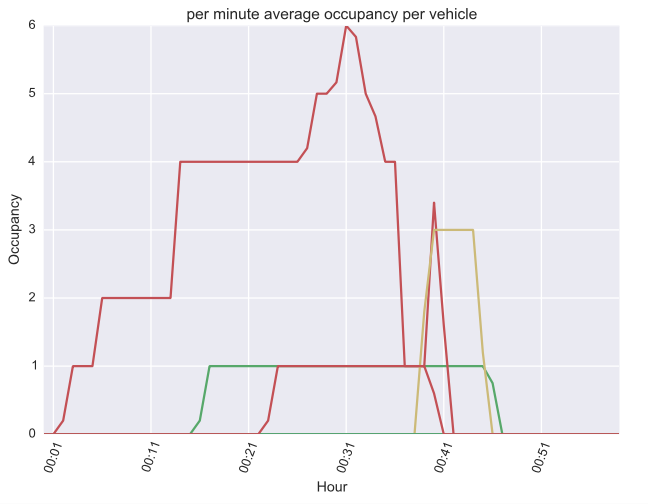
\includegraphics[width=\linewidth]{./images/dem13v10}
  \caption{$dem = 13, |V| = 10$\\ $avgWaitingTime = 3'$\\ $completedBookingsRatio = 0.69$ \\ $averageLoadFactor = 0.03$}
  \label{dem13v10}
\end{subfigure}
\begin{subfigure}[b]{0.48\textwidth}
  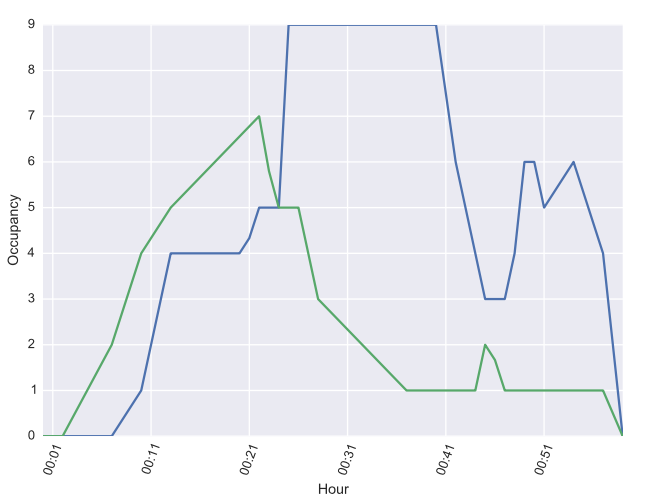
\includegraphics[width=\linewidth]{./images/dem582v}
  \caption{$dem = 58, |V| = 2$\\ $avgWaitingTime = 12'$\\ $completedBookingsRatio = 0.31$ \\ $averageLoadFactor = 0.27$}
  \label{dem58v2}
  \end{subfigure}
  \begin{subfigure}[b]{0.48\textwidth}
  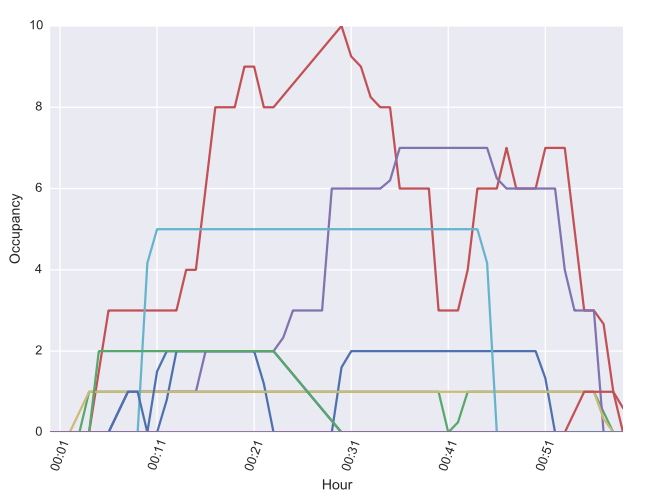
\includegraphics[width=\linewidth]{./images/dem58v10}
  \caption{$dem = 58, |V| = 10$\\ $avgWaitingTime = 5'$\\ $completedBookingsRatio = 0.51$ \\ $averageLoadFactor = 0.15$}
  \label{dem58v10}
\end{subfigure}
%}
\label{extremesimu}
\end{figure}

\subsubsection{Comparison of Scheduling Strategies}
In this section we describe for both dynamic fleet size strategies presented in section \ref{dynamic} what is the output for the fleet size based on the demand density and what are the advantages and disadvantages of those strategies compared to a constant fleet size by analysing the results of the simulations.
\paragraph{First Strategy: Cost Function}
We compute for each $dem \in D =  \{13, 15, 21, 23,$ $25, 27, 31, 36, 40, 46, 58\}$ what is the optimal fleet size $|V^{°}|$ which minimizes the cost function (\ref{costfunction}). We then run a linear regression with the demand density $dem$ as predictors and the optimal fleet size $|V^{°}|$ as dependent variable. We obtain $R^{2} = 0.82$ and we use this linear function which grows from 3 to 8 vehicles to determine at each time of the day what is the optimal fleet size. The adaptive fleet size through the day is shown in Figure \ref{optfleet}.
  
\paragraph{Second Strategy: Maximum Average Waiting Time}
We recall that this strategy implies finding the function of the average waiting time regarding the demand density and the fleet size and then to find the minimum number of vehicles needed to satisfy the level of service constraint. We decide that the $accWaitingTime$ is 6 minutes, as most people are likely to leave the bus station if no bus is coming. In the section \ref{impact} we have explained that we fitted $avgWaitingTime$ to an exponential function. We use therefore this function fit to describe the $avgWaitingTime$ in function of $dem$ and $|V|$. We can therefore for any demand density and fleet size find the $avgWaitingTime$ and choose the fleet which gives an $avgWaitingTime$ under $accWaitingTime$. The result over the day of the optimal fleet size is shown in Figure \ref{optFleet}. We can notice that the number of vehicles varies between 6 and 8 and therefore that more vehicles are needed in order to achieve a given level of service as opposed to the first strategy. It is interesting to observe that this seconds strategy is more sensitive to the changes in demand density and implies therefore more rescheduling events, but that the optimal fleet size range is really smaller than the first strategy. 

\begin{figure}[h] 
  \centering
  \caption{Dynamic fleet size at each hour of the day for the two strategies in function of the demand density divided by ten (for the sake of readability).}
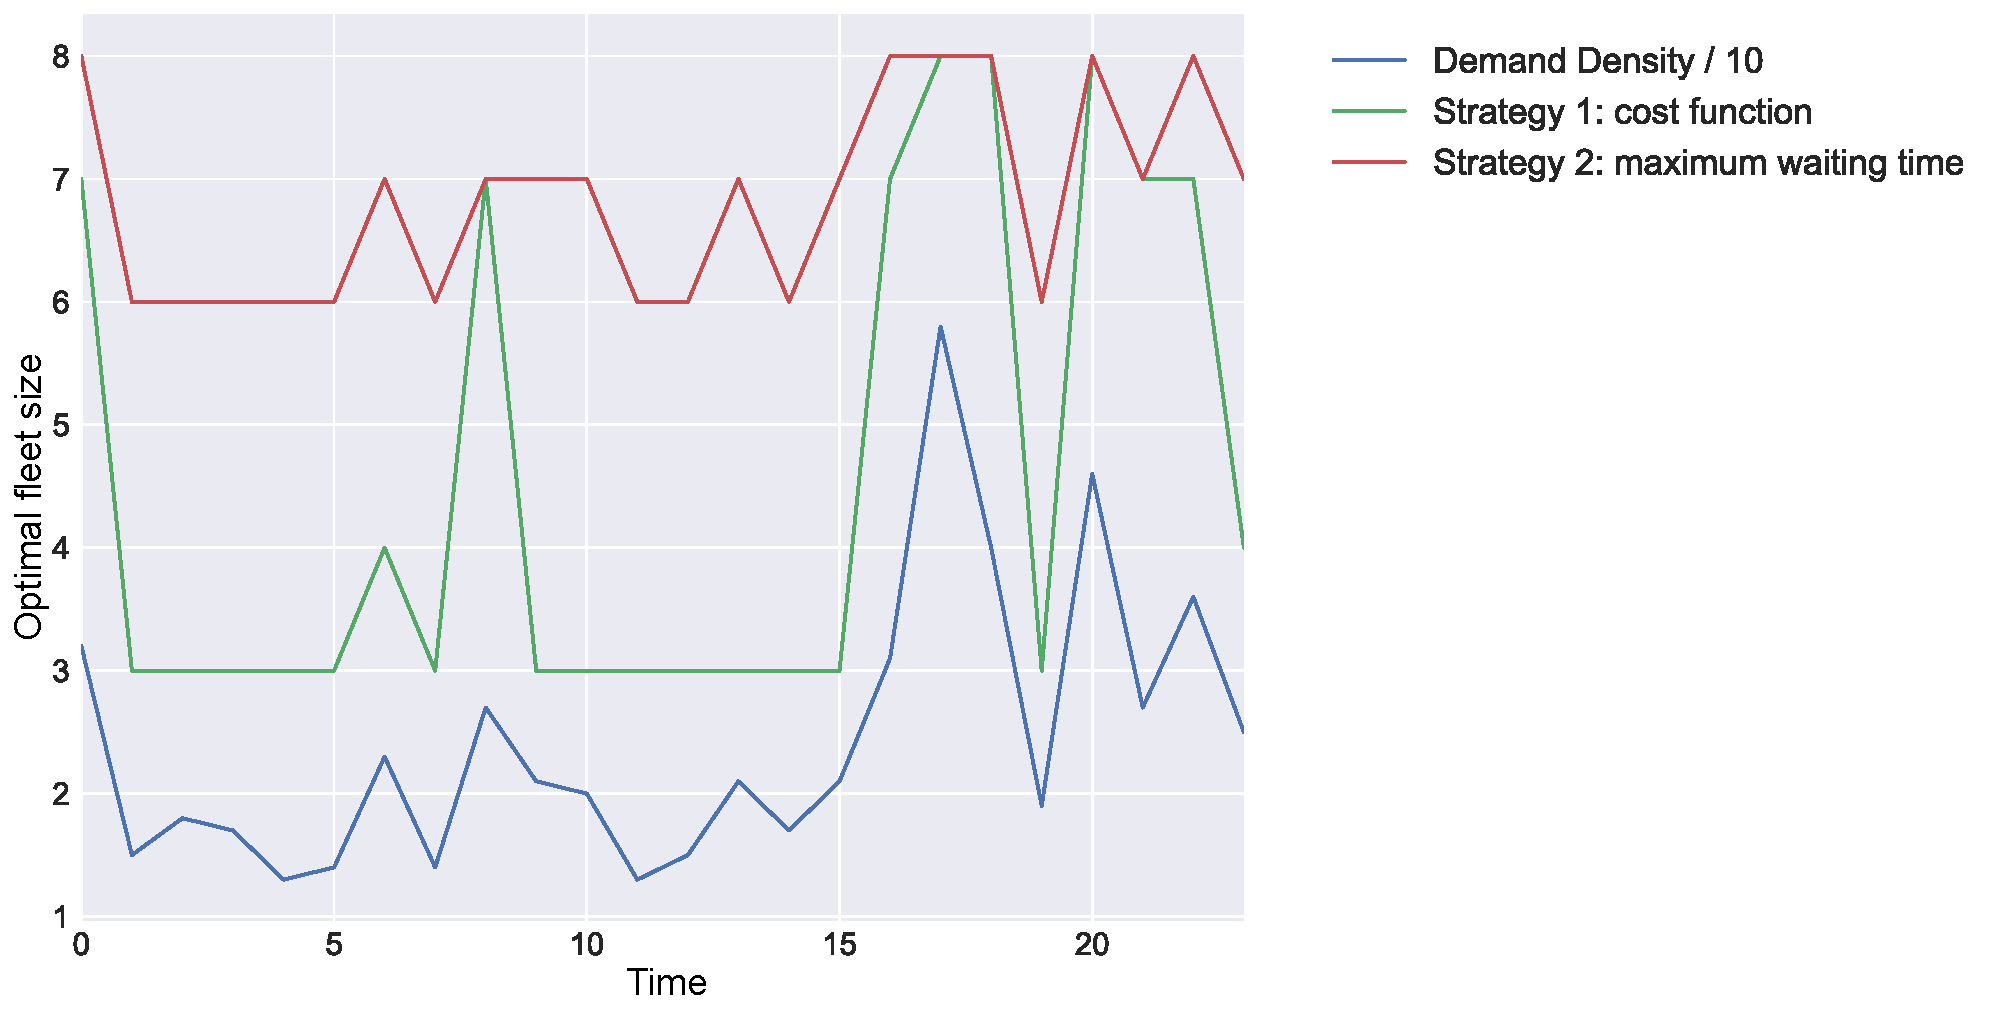
\includegraphics[scale=0.43]{./images/optimalFleet.pdf}
\label{optfleet}
\end{figure}

\paragraph{Comparison of Performance Metrics}
We run the simulations with adapting the fleet size over the scheduling horizon for both strategies. We use the same graph and vehicles' settings as the ones described in section \ref{hwexperiments} with the adaptive waiting time and only mandatory stops. For both of them the maximum optimal fleet size is 8, so we compare those strategies with a constant fleet size of 8 vehicles. The Figure \ref{strategyCompare} illustrates the percentage change of the scheduling  As expected, the battery consumption is lower (14.82 instead of 16.58, as opposed to 16.62 for constant 8 vehicles) for the first strategy as it varies between 3 to 8 vehicles instead of 6 to 8. The $batteryCost$ is therefore only improved by 0.24\% for the second strategy compared to a fixed fleet of vehicles, however the quality of the service offered to the passenger is better. In fact, for the second strategy each booking waits on average 7 minutes compared to 8 minutes for the first strategy and 10 minutes for the constant fleet size. Moreover, the stability of the waiting time is improved as the variance of the waiting times over the completed bookings $waitingStability$ decreases from 307 for the constant fleet size to 91 for the second strategy and 59 for the first one. The cost function strategy has therefore a better $waitingStability$ but a longer $avgWaitingTime$ than the maximum waiting time strategy. However, if we compare the ratio of completed bookings which have a smaller waiting time than 6 minutes over the total number of completed bookings then the second strategy is better than the first one (0.5 instead of 0.48). The usage of vehicles of the second strategy is the most efficient one as the $avgLoadFactor$ is 0.45 instead of 0.3 for the first strategy and 0.25 for the constant fleet size.

\begin{figure}[h] 
  \centering
  \caption{Percentage change of the scheduling strategies' performance metrics relative to the constant fleet of vehicles with mandatory stops.}
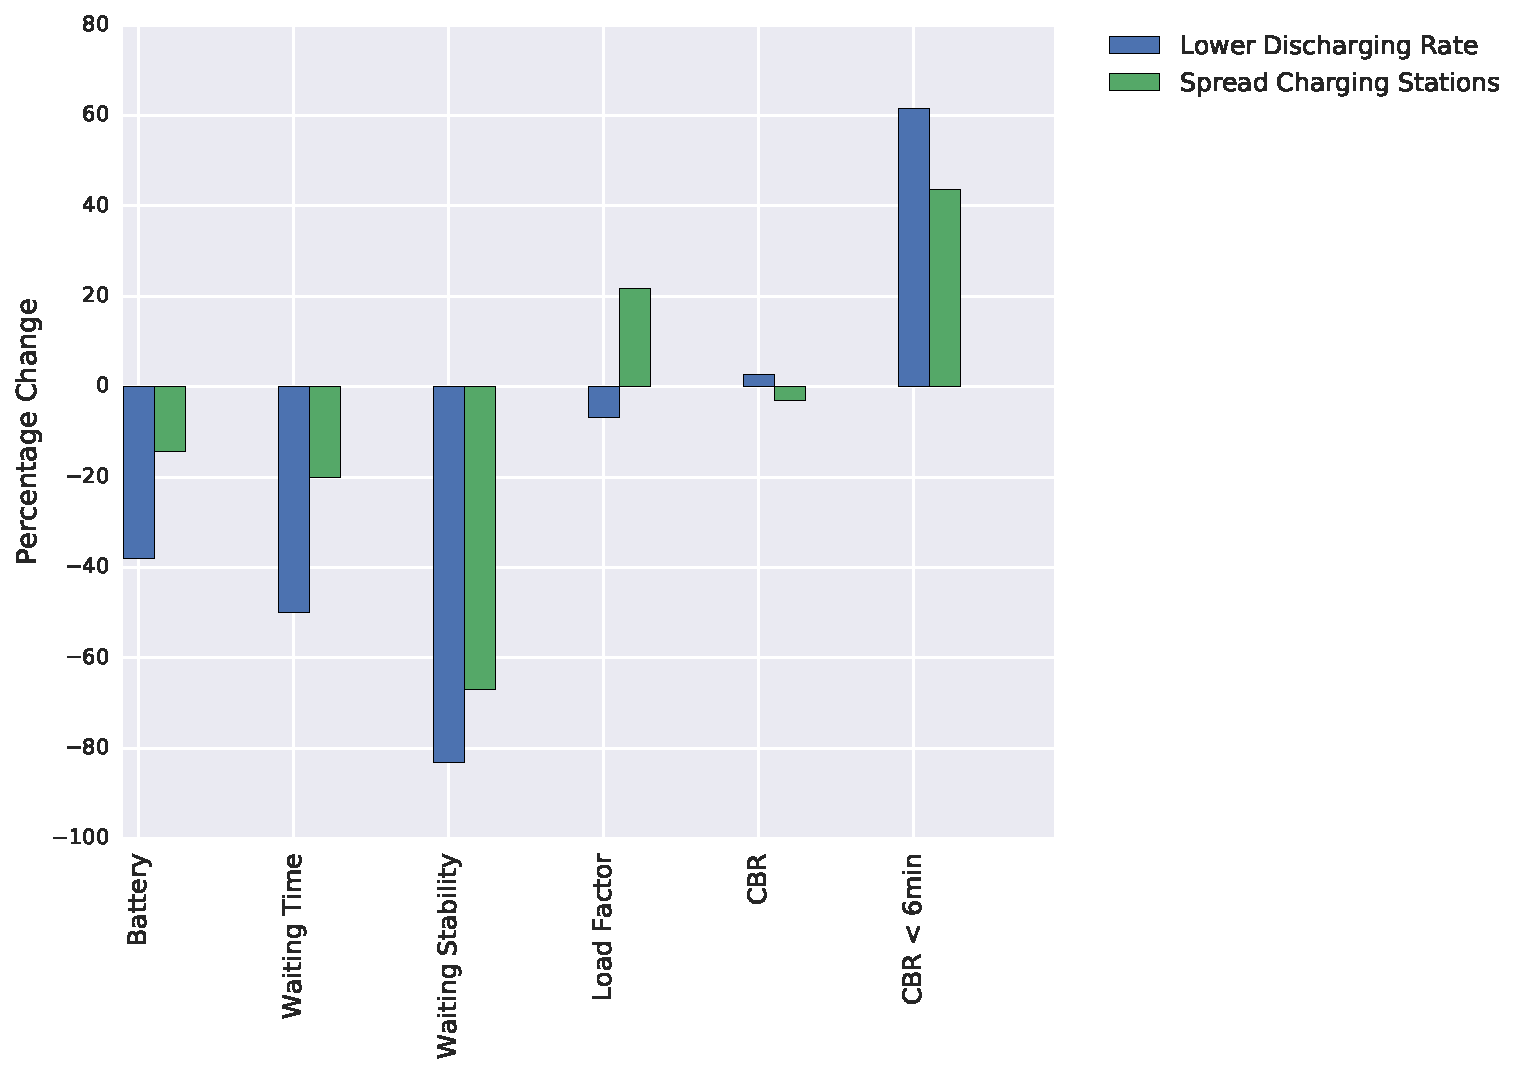
\includegraphics[scale=0.55]{./images/strategyCompare.pdf}
\label{compare}
\end{figure}

\paragraph{Comparison Between Waiting Time and Charging Vehicles}
In order to judge whether the moment a vehicle has been sent to charge was appropriate, we compare the impact it has on the waiting time. We draw therefore a plot that shows the number of charging vehicles on the line and the average waiting time per hour over the day. The average waiting time is normalized between 0 and the fleet size. You can observe in Figure \ref{constantfs} that if the entire fleet size is active at the beginning of the scheduling horizon, then all vehicles will run low on battery approximately at the same time and they will be sent to the charging stations. The waiting time is really low at the beginning but then it increases drastically whilst vehicles are charging and it reflects therefore why the $avgWaitingTime$ and the $stabilityWaitingTime$ are not as good as the metrics obtained when the fleet size is reduced at some hours of the day. In fact, adapting the fleet size through the scheduling horizon allows the vehicles to charge when the demand is lower and to be all available when the demand density is higher and more vehicles are needed. You can see on Figures \ref{batterystrat1} and \ref{batterystrat2} that even though almost all vehicles are active the waiting time still increase around 5pm. It is when the demand density is higher as you can see on Figure \ref{fig:demand}. We can conclude that if the operator has at its disposal only few vehicles then it is really valuable to schedule efficiently when the vehicles should go to charge in order to offer a good quality of service to the clients. 

\begin{figure}
\label{compare2}
  \centering
\begin{subfigure}[b]{0.452\textwidth}
  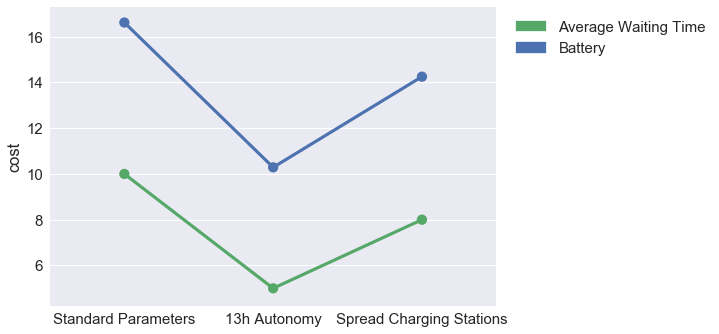
\includegraphics[width=\linewidth]{./images/charge}
  \caption{Constant Fleet Size}
  \label{constantfs}
\end{subfigure}
\begin{subfigure}[b]{0.45\textwidth}
  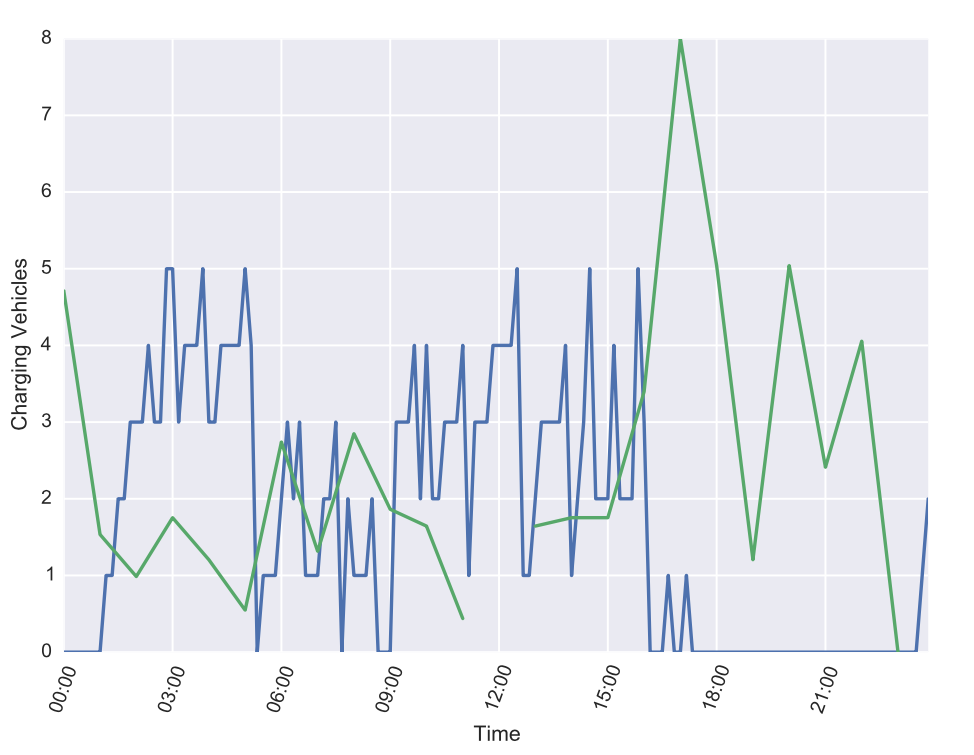
\includegraphics[width=\linewidth]{./images/charge1}
  \caption{Strategy 1: Cost Function}
  \label{batterystrat1}
\end{subfigure}
\begin{subfigure}[b]{0.458\textwidth}
  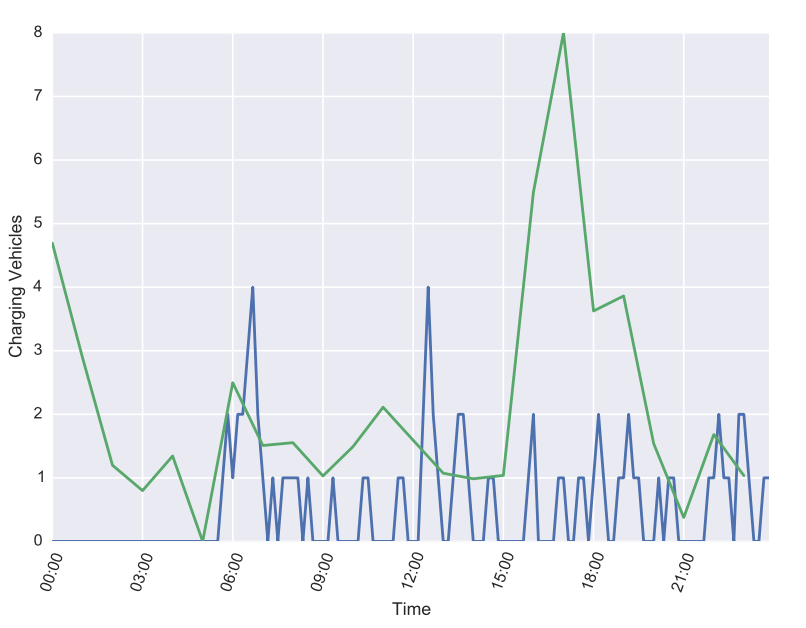
\includegraphics[width=\linewidth]{./images/charge2}
  \caption{Strategy 2: Maximum Waiting Time}
  \label{batterystrat2}
\end{subfigure}
\begin{center}
\vspace{-0.5em}

\includegraphics[scale=0.35]{./images/labels}
\end{center}
\caption{Number of charging vehicles on the line and hourly average waiting time (normalized between 0 and the fleet size) over the simulated day for different scheduling strategies.}
\label{sendtocharge}
\end{figure}

\paragraph{Choice of Scheduling Strategy}
Based on the analysis conducted on the performance metrics of the different scheduling techniques, we can come up with some general advice on which strategy to adopt based on the operator costs' concerns. In fact, the different autonomous models have not the same operating cost: the Institute for Transport Planning and Systems, Swiss Federal Institute of Technology Zürich, conducted a cost-based analysis of autonomous mobility services (see \cite{ethz}). They present a detailed cost estimation for standard transportation systems and future transport modes of automated vehicles. For example, the cost per passenger-kilometer (the average total cost per vehicle and day divided by average passenger kilometers per vehicle and day) varies in function of the vehicle size ans passenger demand. This is illustrated in Figure \ref{passengerkm}. They consider the depreciation, maintenance, cleaning, tires and fuel costs. It might therefore be the case that the operator puts the priority in the customer's level of service as it brings more value than spending a little bit more on the operating cost. In Figure \ref{compare} we can see the improvements of the three different scheduling strategies compared to the constant fleet size. We can conclude that if the fleet operating cost is not a concern we can recommend to consider having optional stops with as many active vehicles as possible. Moreover, if the transportation company owns many vehicles, it might be possible to hold a part of the fleet at the depot and to activate them to replace the vehicles operating on the line which need to be sent to the charging stations. However, if the operating cost of vehicles is high and need to be considered, then it is really valuable to use the adaptive fleet size strategies which reduces the battery consumption (and therefore the kilometers traveled). Moreover, if the operator owns only few vehicles and that the moment to send vehicles to charge is critical as it reduced considerably the fleet size then those strategies are efficient. The first strategy is the best one considering the battery cost and the second one offers a good balance between the level of service offered to the customers and the operating cost.
 
 \begin{figure}[h] 
  \centering
  \caption{Graph illustrating the prices per passenger-km versus number of passengers for traditional and autonomous transit systems (\cite{ethz}).}
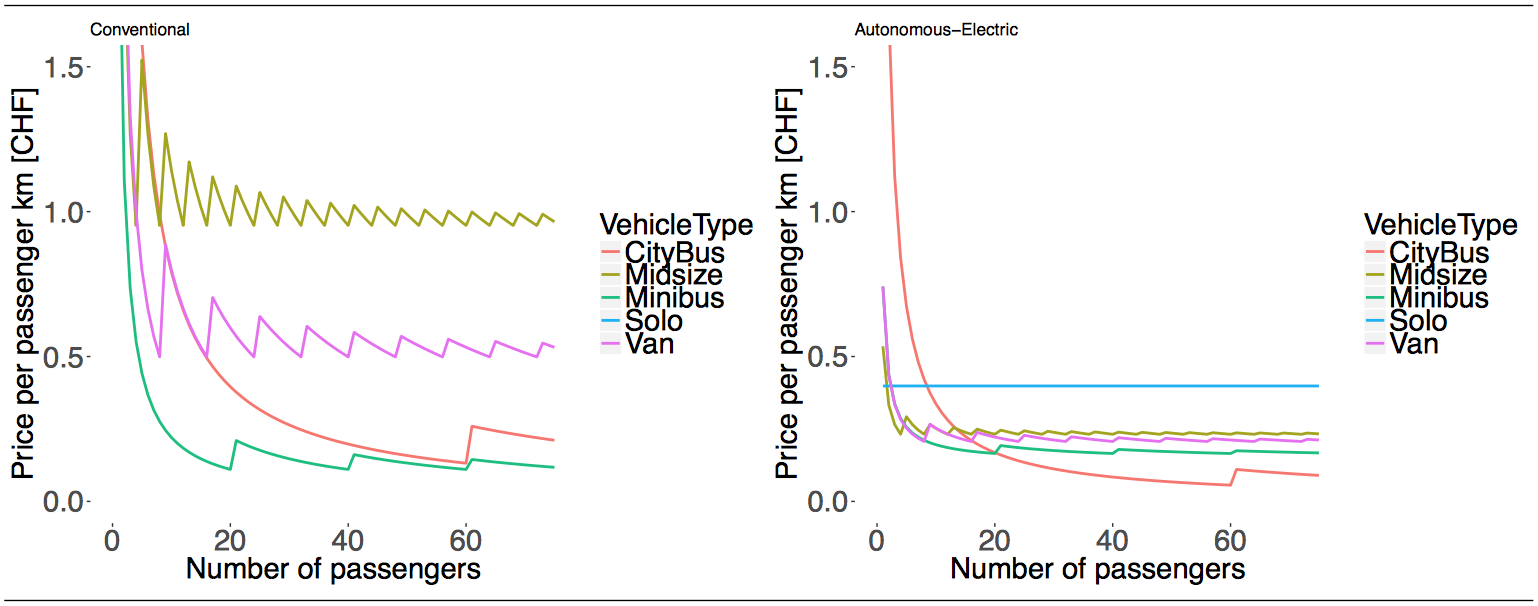
\includegraphics[scale=0.5]{./images/passengerperkmcost}
\label{passengerkm}
\end{figure}


\subsection{Further Scenario Experiments}
All the simulations have been run with exactly the same graph and vehicles configurations. However, it is in the best interest of the operator to know what kind of planning decisions can be made in order to improve the system. As for any transportation service, there are some compromises to take a priori concerning the overall money spent on the fixed line design and vehicles, allowing a reasonable return on investment. We run therefore two additional simulations changing the charging station places in section \ref{spreadcharging} and the vehicles' battery consumption model in section \ref{batterycons}.

\subsubsection{Autonomous Charging Stations}\label{spreadcharging}
In current cities where vehicles are operating, the charging stations are located all at the same place. In fact, they are at the depot where shuttles are stored and an employee needs to manually put them on charge. The National Center for Transit Research (NCTR), University of South Florida, published a report summarizing the state of public transportation vehicle automation and the characteristics of the latest two autonomous electric shuttles (see \cite{nctr}). Each charging station costs 20'000 Euros (22'558 USD) whilst each vehicle cost approximately 200'000 to 220'000 Euros. However, some new technologies are emerging in this sector which do not imply any human help. For example Plugless offers an autonomous wireless charging station, for the same charging power (3.3kW, see \cite{plugless}) which cost 5'999 USD. We can therefore envision a future system making use of these new technologies. It would be a line with autonomous charging stations spread along the loop instead of one single depot where they need to go to charge. In order to measure how it would ameliorate the transportation system, we change the graph by placing 13 charging on the loop. We run a simulation for a constant fleet size of 8 vehicles and only mandatory stops and compare it to the scenario with the charging stations at one place. The improvements can be visualized in Figure \ref{batterycompare}. The $batteryCost$ drops from 16.62 to 14.25 (-14 \%) as vehicles do not need to stop operating and travel long distances to the single charging station point. The $avgWaitingTime$ is improved as well from 10 minutes to 8 minutes and especially the completed bookings ratio which have a waiting time under 6 minutes grows from 0.47 to 0.56. You can observe on Figure \ref{spread} that the waiting time increases again when vehicles need to go to charge as it happens at the same time when they run low on battery so we could even obtain better results if a dynamic fleet size scheduling strategy is used. 

\begin{figure}
  \centering
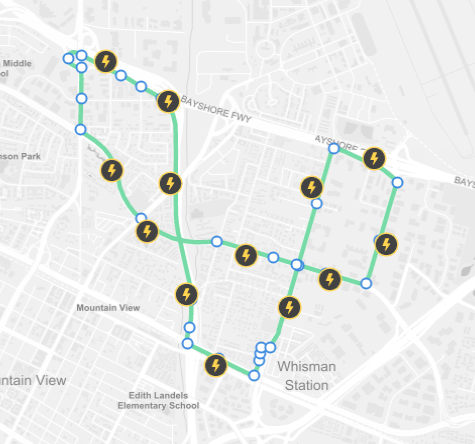
\includegraphics[scale=0.5]{./images/manycharging}
  \caption{Fixed line scenario with spread autonomous charging stations.}
\label{manycharging}
\end{figure}

\begin{figure}
  \centering

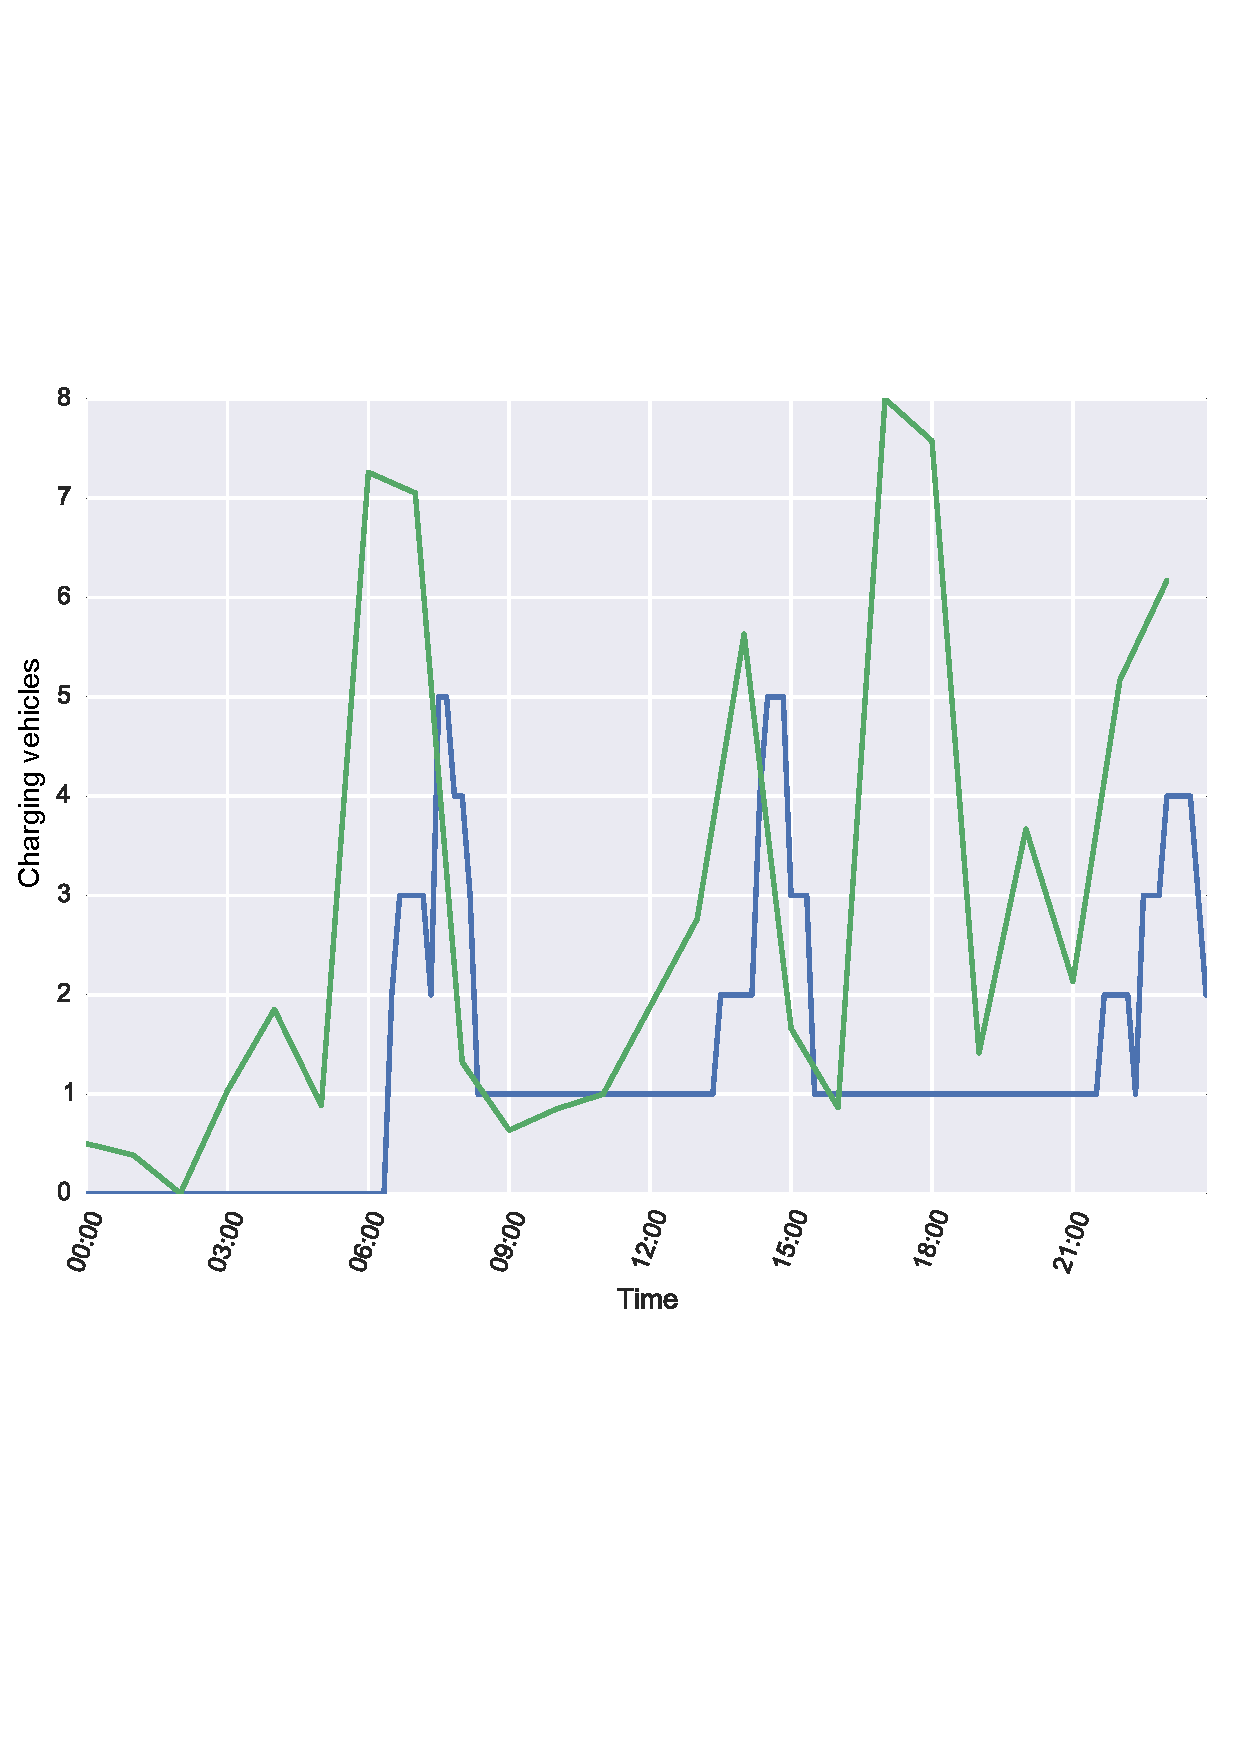
\includegraphics[scale=0.5]{./images/spreadcharging.pdf}
 \caption{Number of charging vehicles on the line and hourly average waiting time (normalized between 0 and the fleet size) over the simulated day for a line with spread charging stations.}
\label{spread}
\end{figure}


\subsubsection{Battery Consumption}\label{batterycons}
The different shuttle models available today on the market have different battery performances. In fact, as detailed in the NCTR report (\cite{nctr}) mention the difference between autonomous shuttles of two different manufacturers: EasyMile and NAVYA. The latest model EZ10 from the French company EasyMile has a an autonomy up to 14 hours, whilst the ARMA electric bus from an other French company NAVYA has an autonomy ranging from 5 to 12 hours, depending on the charging system and the battery capacity. Operators are faced to choose one model or the other and will always be confronted to a growing offer as other manufacturers are currently developing new autonomous electric vehicles. It is therefore important for them to know what kind of benefits a better battery can bring to the overall system's performance. We modify the discharging ratio $\beta$ which was equal to 1 to 0.65. The battery consumption function \ref{vehicleequation} decreases therefore slower and vehicles have a longer autonomy corresponding to approximately 13 hours. We run a simulation with the updated discharging function for a constant fleet size of 8 vehicles. During the simulated day vehicles need to be sent to charge only once instead of twice. The $batteryCost$ is reduced from 16.62 to 10.29, decreasing by 38\%, which is coherent as we reduced the battery discharging ratio $\beta$ by 35\%. The 3\% difference is explained by the fact that when vehicles are sent to charge they do not wait at each stop any more and therefore consume more battery. The interesting performance metric which is improved is the average waiting time: in fact, it is reduced from 10 minutes to 5 minutes. The impact of sending vehicles to charge is therefore not negligible as it has a considerable negative effect on the $avgWaitingTime$, the $stabilityWaitingTime$ and the $completedBookingsRatio < 6min$. 

\begin{figure}
  \centering
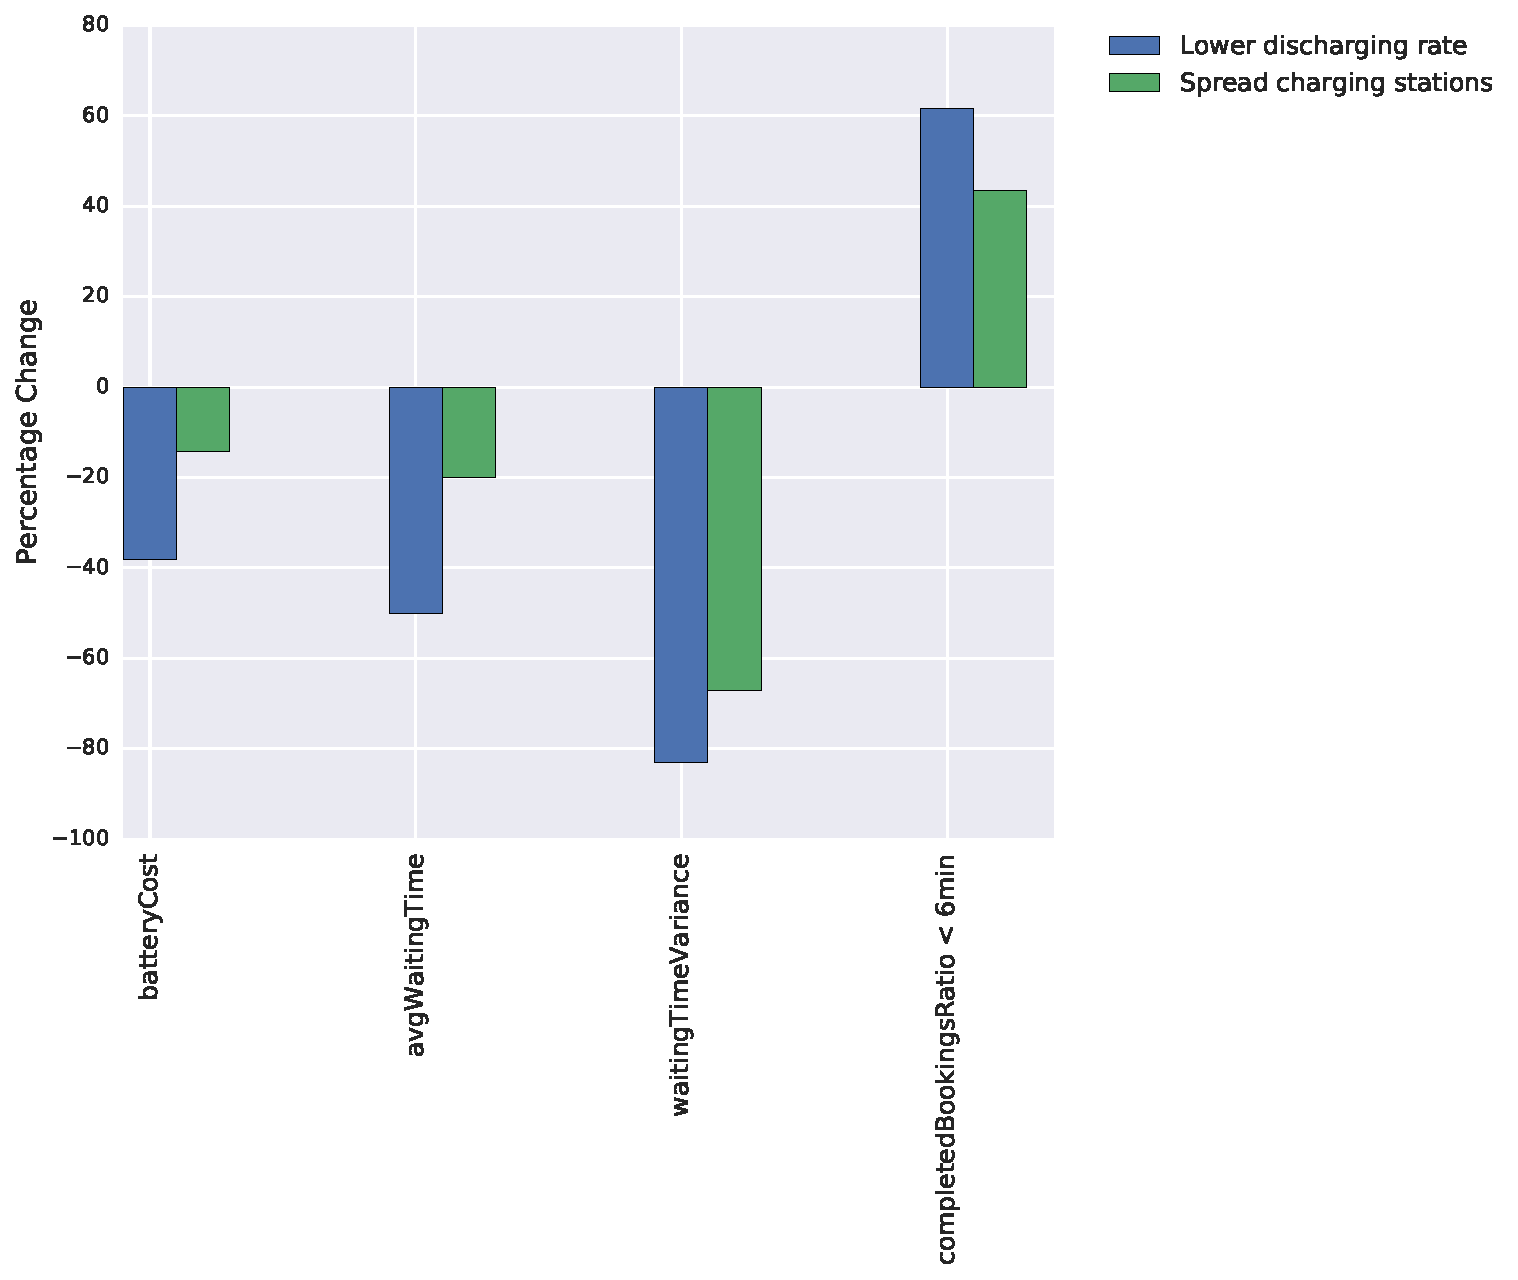
\includegraphics[scale=0.55]{./images/batteryCompare.pdf}
  \caption{Percentage change of the scheduling strategies' performance metrics relative to the constant fleet of vehicles with mandatory stops.}
\label{batterycompare}
\end{figure}

\begin{sidewaystable}
\center
\pgfplotstabletypeset[
col sep = comma,
string replace*={_}{\textsubscript},
every head row/.style={before row=\toprule,after row=\midrule,
typeset cell/.code={
            \ifnum\pgfplotstablecol=\pgfplotstablecols
            \pgfkeyssetvalue{/pgfplots/table/@cell content}{\rotatebox{90}{##1}\\}%
            \else
            \pgfkeyssetvalue{/pgfplots/table/@cell content}{\rotatebox{90}{##1}&}%
            \fi
            }
},
every last row/.style={after row=\bottomrule},
display columns/0/.style={string type,column name={}}
]
{avg_value.csv}
\caption{Performance metrics of all simulations run over one simulated day for the different scheduling strategies.}
\end{sidewaystable}

\section{Conclusion}\label{conclusion}
\subsection{Summary}\label{summary}
\subsection{Future Work}\label{futurework}

\newpage
\bibliographystyle{apalike}
\bibliography{/Users/prisca/Documents/Final_Report/bibliography/bibliography}

\end{document}
